% \section{Software Requirements Specification}

\section{Theoretischer Teil}

\subsection{\textbf{Einleitung}}
Mit dem Zeitpunkt der Erfindung des Computers ist eine Aufgabe der Informatik eine Möglichkeit für die Kompression und Kodierung von Daten zu finden. Spätestens mit der Erfindung von grafischen Ausgabegeräten wie Monitor und Drucker ist der Bedarf an einer effizienten und platzsparenden Speicherung, sowie Übermittlung, von Daten stetig gewachsen. In nahezu allen technischen Bereichen werden heutzutage digitale Bilder verwendet. Neben der digitalen Fotografie, der Archivierung von Bilddokumenten und der technischen Qualitätskontrolle kommen digitale Bilder zum Großteil auf Webseiten zum Einsatz. Würden hier dieselben Qualitätsansprüche an digitale Bilder gestellt werden, wie man sie an die klassische Fotografie stellt, würden enorme Datenmengen von mehreren Megabyte pro Bild entstehen. Deshalb ist eine effiziente und platzsparende Kompression unerlässlich. Diese Arbeit geht kurz auf die Definitionen und Grundlagen der Bildkompression ein und veranschaulicht dies durch die Quantisierung in drei verschiedenen Applikationen. Eine dieser drei Applikationen wird im Laufe dieser Arbeit mit den gewonnenen Erkenntnissen verbessert und vereint die positiven Eigenschaften der anderen Applikationen. (1)
%Dieses Dokument dient als Dokumentation des berufsbegleitenden Studienganges, Kommunikations- und Medieninformatik des Matrikel 13, mit der Programmierung einer APP zur Kompression von Bilddaten. Es setzt dabei die Rahmenbedingungen fest.
\subsection{\textbf{Was ist Bildkompression?}}
Doch zunächst klären wir was unter Bildkompression verstanden wird. Wie jede Datenkompression, beruht auch die Bildkompression darauf aus dem ursprünglichen Datensatz Daten zu entfernen, deren Verlust kaum wahrnehmbar ist oder welche vollständig rekonstruierbar sind. Datenkompression ist ein Verfahren zur Reduktion des Speicherbedarfs von Daten, zu einem solchen Verfahren gehören logischerweise Methoden zur Reduktion des benötigten Speicherbedarfs (Kompression) und zur Wiederherstellung dieser Daten in die ursprüngliche Form (Dekompression). Nach jeder Kompression gilt immer folgende Gleichung:

\begin{center}
\textit{komprimierte Datei = Originaldatei - Redundanz}
\end{center}

„Unnötige“ Daten kann man im allgemeinen als Redundanz bezeichnen, also Daten, die für die eigentliche Information nicht wichtig sind, da sie entweder für den Menschen nicht wahrnehmbar sind oder sie komprimiert werden können (z.B. wiederkehrende Muster). Das bedeutet im Umkehrschluss, dass Daten die keine Redundanzen enthalten nicht komprimiert werden können. Dasselbe gilt natürlich für Daten deren Redundanzen nicht erkannt werden. Wird die unkomprimierte Datenmenge durch einen Wert dividiert, so erhält man die komprimierte Datenmenge. Dieser Wert wird als Kompressionsrate bezeichnet. „Üblich ist die Angabe als Quotient in der Form x : 1. Es ergibt sich also die Gleichung:

\begin{center}
\textit{Datenmenge(kompr.) = Datenmenge(unkompr.) : Kompressionsrate}
\end{center}

Ein Beispiel: 
Die unkomprimierte Datenmenge beträgt 300 MB und die Kompressionsrate beträgt 20 : 1.
Somit ergibt sich für die Datenmenge(kompr.) = 300 MiB : 20 : 1 = 300 MiB : 20 = 15 MiB (2)

\subsection{\textbf{Menschliches Sehen}}
Welcher Zusammenhang besteht nun zwischen Redundanz, also „unnötigen“ Daten und dem menschlichem Auge. Im Auge bildet die Linse das Originalbild auf Netzhaut (Retina) ab. Diese enthält Fotorezeptoren, welche aus rund 130.000.000 und 7.000.000 Zäpfchen besteht. Die Stäbchen registrieren Intensität (Hell-Dunkel-Verhältnis) , wohingegen die Zäpfchen für die Farbregistrierung zuständig sind, je ein Zäpfchentyp für Grün, Rot, Blau. Durch Mischung der drei RGB-Farbkanäle lässt sich redundanzarm ein visueller Eindruck erzeugen, der dem natürlich wahrgenommenen Bild recht ähnlich ist. Das menschliche Auge kann circa 60 verschiedene Grautöne unterscheiden, daher reichen $2^{8}$ = 256 Grauwerte aus um einen visuellen Eindruck zu erreichen. 

\subsection{\textbf{Digitalisierung}}
Um analoge Bilder in digitalen Systemen nutzen zu können müssen diese zunächst in eine geeignete numerische Darstellung gebracht werden, dazu sind der Definitionsbereich, d.h. die Menge der erlaubten Punkte (Pixel) der Wertebereich (Grau- / Farbwerte) in endlich viele Intervalle aufzuteilen.
Dieser Gesamtvorgang wird als Digitalisierung bezeichnet. Die Digitalisierung des Definitionsbereiches wird als Rasterung (Scanning) und die Digitalisierung des Wertebereiches wird als Quantisierung (Sampling) bezeichnet.

\subsubsection{Bilderzeugung}
Prinzipiell wird ein Objekt bei der Bilderzeugung über eine Linse auf der Bildebene abgebildet (siehe Abbildung: \ref{fig:bilderzeugung_steph}). Hier setzt die Digitalisierung ein. In der Realität können nur Bilder endlicher Ausdehnung behandeln werden, daher muss das Bild oder besser der Bildausschnitt gefenstert werden (Fensterung). Außerdem können nur endlich viele Signale verarbeitet werden, daher wird die Projektion des Objektes auf der Bildebene abgetastet (Abtastung/Sampling). Die einzelnen Intensitätswerte werden in einer Bildmatrix übernommen.

\begin{figure}[h]
	\centering
		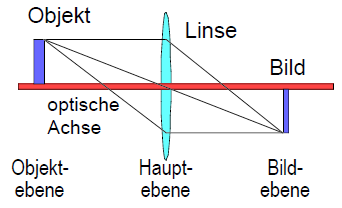
\includegraphics[width=0.6\textwidth]{img/prinzip_bilderzeugung.png}
	\caption[Prinzip der Bilderzeugung]{Prinzip der Bilderzeugung}
	\label{fig:bilderzeugung_steph}
\end{figure}

Es können des Weiteren nur endlich viele Signalamplituden verarbeitet werden (Quantisierung), daher werden den einzelnen Bildpunkten (Pixeln) konkrete Werte zugeordnet. Wie in Abschnitt 3 werden die Intensitätswerte durch Graustufen dargestellt, somit werden den Pixeln also konkrete Graustufen zugeordnet (siehe Abbildung: \ref{fig:abtastung_steph}). Dasselbe Prinzip gilt auch für die erwähnten Farbwerte.

\begin{figure}[h]
	\centering
		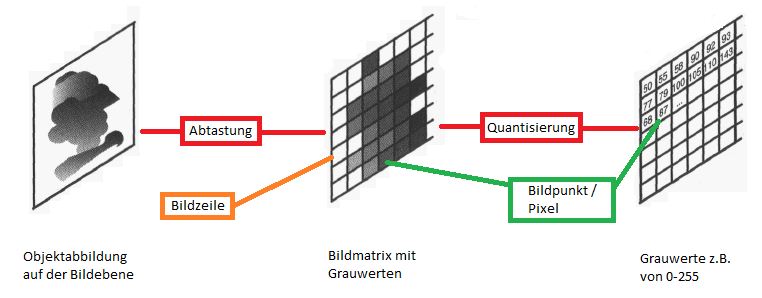
\includegraphics[width=0.8\textwidth]{img/prinzip_abtastung.png}
	\caption[Prinzip der Abtastung und Quantisierung]{Prinzip der Abtastung und Quantisierung}
	\label{fig:abtastung_steph}
\end{figure}


\subsubsection{Abtastung}

Die Projektionsfläche auf der Bildebene wird durch ein regelmäßiges Raster von Photosensoren abgetastet. Je nach Dichte der Abtastpunkte pro Flächeneinheit entsteht ein hochaufgelöstes oder ein "grobkörniges" Bild. Unter Abtastung versteht man im Allgemeinen „die Erfassung eines zeitkontinuierlichen analogen Signals in bestimmten Zeitabständen. Zu diesem Zweck wird das Analogsignal zu den Abtastzeitpunkten t1, t2 usw. abgetastet und der dabei erhaltene Signalwert einer Halteschaltung zugeführt. Die Abtastung erfolgt in aller Regel gemeinsam mit der Spannungshaltung in einer Abtast- und Halteschaltung, Sample and Hold. Die Zeitabstände zwischen den einzelnen Abtastungen ist die Abtastrate.“ (3)
Bei biologischen Augen sind die Photorezeptoren in einer "Wabenstruktur" angeordnet. 
Auch bei neueren technischen Entwicklungen (elektronische Chip- Augen) werden hexagonale Gitter benutzt. Vorteile sind hier die bessere Chip-Flächenfüllung bei integrierter Signalverarbeitungselektronik, sowie die homogenen Pixelabstände. Andere technische bildverarbeitende Systeme benutzen (heute) fast ausschließlich ein kartesisches Basisgitter für das Bildraster, welches aus rechteckigen bzw. quadratischen Pixeln besteht. Der Vorteil eines kartesischen Rasters liegt in der einfachen mathematischen Behandlung als Matrix, jedoch sind in diesem Raster nicht alle Pixelabstände homogen. Sie sind also inhomogen (siehe Abbildung: \ref{fig:bildraster_steph}).

\begin{figure}[h]
	\centering
		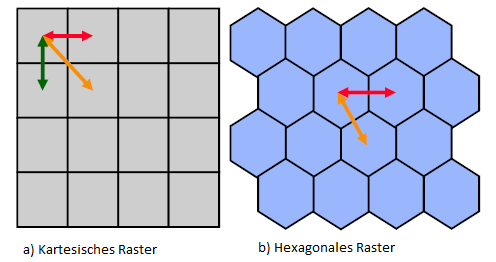
\includegraphics[width=0.8\textwidth]{img/vergleich_bildraster_Steph.png}
	\caption[Vergleich Bildraster]{Vergleich Bildraster}
	\label{fig:bildraster_steph}
\end{figure}

Die Größe der Gittermaschen, die über das Urbild gelegt werden, hat einen entscheidenden Einfluss auf die Qualität des digitalisierten Bildes. Bei der Wahl eines zu groben Rasters gehen Details verloren oder feine Bilddetails werden verfälscht wiedergegeben. Bei einem zu feinen Gitter steigt die Auflösung, aber auch die Dateigröße. Da eine zu grobe Rasterung zu einer Verschmelzung der Objektdetails führen kann gilt folgendes:
„Die Rasterweite eines Bildes darf nicht gröber sein als die halbe geometrische Ausdehnung des kleinsten noch abzubildenden Objektdetails.“ (3)
Ein ähnliches Prinzip gilt für die Abtastung. Hier greift das Nyquist-Shannonsche Abtasttheorem, welches besagt, dass ein kontinuierliches Signal (mit einer Maximalfrequenz $ f_{\mathrm{max}} $ ) mit einer Frequenz größer als 2 * $ f_{\mathrm{max}} $ abgetastet werden muss, damit aus dem so erhaltenen zeitdiskreten Signal das Ursprungssignal ohne Informationsverlust rekonstruiert werden kann. 

\begin{figure}[h]
	\centering
		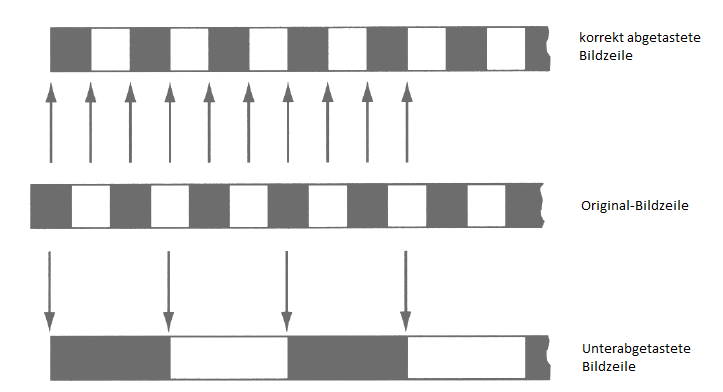
\includegraphics[width=0.8\textwidth]{img/abtastung_steph.png}
	\caption[Abtastung]{Abtastung}
	\label{fig:abtastung2_steph}
\end{figure}

In Abbildung: \ref{fig:abtastung2_steph} erkennt man, dass die Abtastrate doppelt so groß wie die Detailfrequenz ist und somit das Original wiedergegeben werden kann. Bei zu geringer Abtastrate wird das Original verfälscht. Über diesen Effekt, der Unterabtastung, muss man sich klar machen, dass je nach Abtastrate auch noch viel drastischere Effekte eintreten können: Wenn der Abtastpunkt etwa alle zwei Kästchen kommt (also Detailfrequenz = Abtastfrequenz) und immer im "Schwarzen" des Originals liegt, dann wird der Sample\& Hold -
Wert immer schwarz sein (siehe Abbildung: \ref{fig:alias_steph} Alias-Effekt)! Dies ist der Effekt des Aliasing: Frequenzen, die für die Abtastrate zu hoch sind, sehen so aus wie tiefe. Die hohen Frequenzen geben sich sozusagen als jemand anderes aus, daher die Bezeichnung Alias. 

\begin{figure}[h]
	\centering
		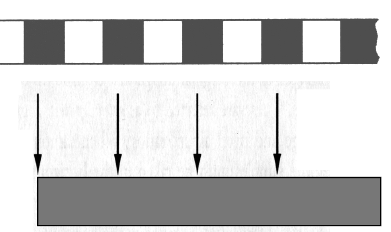
\includegraphics[width=0.8\textwidth]{img/alias_steph.png}
	\caption[Alias-Effekt]{Alias-Effekt}
	\label{fig:alias_steph}
\end{figure}

\subsubsection{Quantisierung}
Quantisierung ist, wie in den vorherigen Abschnitten beschrieben Teil der Digitalisierung von analogen Signalen. Mit dem Begriff Quantisierung wird die Zuordnung der digitalisierten Grauwerte zu den Pixeln bezeichnet. Als Werte werden meist die natürlichen Zahlen von 0 bis 255 verwendet. Neben der Rasterfeinheit wird die Bildqualität durch die Anzahl der Gaustufen zwischen Schwarz und Weiß bestimmt. Eine Reduzierung der Graustufen eines Grautonbildes führt zu größeren homogenen Flächen mit störenden Kanten. Die meisten Bildverarbeitungssysteme besitzen 256 oder sogar 1024 Graustufen. Man sagt auch, sie können mit 8 Bit bzw. 10 Bit quantisieren (${2}^8$ = 256; ${2}^{10}$ = 1024). Die Digitalisierung von Farbbildern entspricht der von Grautonbildern mit dem einzigen Unterschied, dass das Farbbild in seine Rot-, Grün- und Blauanteile durch Filter zerlegt Wird. Für jeden Farbanteil gibt es eine eigene Bildmatrix. Die Rot-, Grün- und Blaumatrizen lassen Sich zum Originalbild kombinieren. Da für jede der drei Matrizen 256 bzw. 1024 Grauwerte für die Quantisierung zur Verfügung stehen, beträgt die Zahl der theoretisch realisierbaren Farbwerte 16,7 Millionen (24bit) bzw. 1,07 Milliarden (30bit). Bilder stellen große Dateien dar, die in bestimmter Weise organisiert sind. Dabei wird besonders viel Wert auf die Datenreduktion gelegt, ohne die Qualität der Bilder wesentlich oder überhaupt nicht zu mindern. Neben der Datenreduktion durch die Momentanwertabtastung, bei der die Datenreduktion nur durch Verlust von Daten auftritt. Eine sehr einfache Methode zur Datenreduktion demnach die Quantisierung, bei der die Genauigkeit reduziert, wird mit der die Daten abgespeichert werden.


\subsection{\textbf{Kompressionsarten}}

Bei den Kompressionsverfahren unterscheidet man zwischen drei verschiedenen Arten:
\begin{itemize}
\item  Signalkompression: Die Reduzierung der Redundanz im Signal wird hierbei durch die Betrachtung jedes einzelnen Pixels, unabhängig von allen anderen Pixeln erreicht.
\item  Umgebungsbasierte Kompression: Die Redundanz zwischen benachbarten Pixeln wird reduziert, in dem eine Pixelfolge betrachtet wird.
\item Wahrnehmungsorientiertenkompression: Die Reduktion der Information, die für die Wahrnehmung der Bilddateien relevant ist. Zum Beispiel die Reduktion des Wertebereichs auf 64 Helligkeitswerte mit der Begründung, dass rund 60 Werte durch den Betrachter unterschieden werden können. (4)
\end{itemize}
Verfahren, die einer der ersten beiden Strategien folgen, führen zu einer Verlustfreie Kompression. Durch die Reduktion von Informationen (Wahrnehmungsorientierten-kompression) können höheren Kompressionsraten erreicht werden. Aufgrund der sehr hohen Kompression gehen hier Daten verloren und die Rekonstruktion ist nur näherungsweise möglich, daher spricht man von einer verlustbehaftete Kompression.

\subsubsection{Verlustbehaftete Kompression}
Diese Kompressionsart wird verwendet, wenn Bildinformation übertragen werden müssen, bei der Details nicht den Informationsgehalt des Bildes bestimmen. Hier findet eine Reduktion der Bilddaten statt, sodass das Ursprungsbild nicht 1:1 wiederherstellbar ist. Die Fehler, die bei zu starker Datenreduktion sichtbar werden, nennt man Artefakte. Einsatzgebiete sind z.B. digitales Fernsehen, Telekonferenzen, Bilder im Internet. Bei Netzwerken wie dem Internet kommt noch hinzu, dass die Übertragungsgeschwindigkeiten meist sehr niedrig sind, und da verlustbehaftete Kompression vor allem bei True-Color Bildern eine viel höheren Kompressionsfaktor erreicht als die Verlustfreie, wählt man hier diese Kompressionsart. Hier gilt der Grundsatz „Speed before Quality“. Formate die verlustbehaftete Kompression unterstützen sind z.B.: GIF, JPEG, Wavelet.
\subsubsection{Verlustfreie Kompression}
Wie vom Namen her zu raten ist, soll bei diesem Verfahren keine Information verloren gehen. Die verlustfreie Kompression kommt vorwiegend in der professionellen Bildbearbeitung zum Einsatz, wo mit teureren, schwer zu beschaffenden oder aufwendig zu berechnenden Bilddaten gearbeitet wird. Hier ist jede Bildinformation wichtig. Es findet also keine Reduktion der Daten statt. Im Gegensatz zur verlustbehafteten Kompression gilt hier „Quality before Speed“. Einsatzgebiete sind z.B. Satellitenbilder, medizinische oder künstliche Bilder.
Formate die verlustfreie Kompression unterstützen sind z.B.: BMP, GIF, PNG, JPEG, TIF.
Das Prinzip beruht darauf, die Daten anders als vorher zu organisieren, indem Wiederholung von Strukturen erkannt und hierarchisch dargestellt werden. Zum Beispiel wird eine sich wiederholende Bitfolge einmal in einer Art Wörterbuch abgelegt und dann nur noch durch ihre Nummer repräsentiert.


\FloatBarrier %Fließumgebungsbarriere


\subsubsection{Vergleich Tabellarisch}
Die wichtigsten Unterschiede zwischen den beiden Verfahren sind aus dem Qualitätsunterschied eines Bildes, vor einer Kompression und nach der wieder Dekomprimierung des gleichen Bildes, sichtbar (siehe Abbildung \ref{fig:vergleich_steph}Tabellarischer Vergleich). 

\begin{table}[h]
\begin{tabular}{|c|c|}
\hline
 \textbf{Verlustfreie} & \textbf{Verlustbehaftete} \\
 \hline
 + keine Zerstörung der Bilddaten & + hohe Kompressionsrate erreichbar \\
 + Dekompression rekonstruiert & - Verringerung der Informationsdichte \\
 + Ursprungsdaten vollständig & -Dekompression rekonstruiert \\
 - niedrige Kompressionsrate erreichbar & - Ursprungsdaten nicht vollständig \\
 - hoher Übertragungsaufwand & + niedriger Übertragungsaufwand \\
 \hline

\end{tabular}
 \caption[Tabellarischer Vergleich]{Tabellarischer Vergleich}
	\label{fig:vergleich_steph}
\end{table}



\subsection{\textbf{Skalare Quantisierung}}
Die skalare Quantisierung ordnet jedem Signalwert einen quantisierten Wert aus einer endlichen Wertemenge zu. Die Zuordnung erfolgt dabei im einfachsten Fall linear auf Basis eines Rasters mit Intervallen fester Länge. Alle Samples innerhalb eines bestimmten Intervalls werden dabei auf denselben quantisierten Wert abgebildet, wodurch verlustbehaftete Datenkompression entsteht. Anstelle eines festen Rasters können auch unterschiedliche Intervallbreiten gewählt werden, um bestimmte Werte stärker zu quantisieren als andere. Dies kann beispielsweise Sinn machen, wenn sich dadurch Einschränkungen der menschlichen Wahrnehmung ausnutzen lassen und wird als nichtlineare Quantisierung bezeichnet. 

\subsection{\textbf{Vektorquantisierung}}
Die Vektorquantisierung berücksichtigt n Signalwerte gleichzeitig, die als Vektor des n-dimensionalen Raums aufgefasst werden. Wie die skalare Quantisierung stellt auch die Vektorquantisierung einen verlustbehafteten Vorgang dar. Ein Vektorquantisierer der Dimension n und Größe s bildet Eingabevektoren auf eine endliche Menge C ab, die aus s Ausgabevektoren besteht. Für die Wahl der Ausgabevektoren aus C können verschiedene Kriterien herangezogen werden. Im einfachsten Fall kommt das euklidische Abstandsmaß der Vektoren zum Einsatz. Die Menge C der Ausgabevektoren wird als Codebuch bezeichnet. Die größte Herausforderung bei der Vektorquantisierung ist die Wahl eines geeigneten Codebuchs. Dieses muss in einer Trainingsphase mit Hilfe charakteristischer Signalvektoren optimiert und so an typische Signalstatistiken angepasst werden. Ein verbreiteter Algorithmus zur Codebuch-Erstellung ist der LBG-Algorithmus.

\subsection{\textbf{Das RGB-Farbmodell}}
Um Farben quantitiv beschreiben zu können, gibt es sogenannte Farbmodelle. Da für die Beschreibung des folgenden Verfahrens zur Farbquantisierung vorwiegend das RGB-Farbmodell genutzt wird, soll es hier genauer erläutert werden. Alle Farbstufungen entstehen beim RGB-Farbmodell durch Mischen der drei Grundfarben Rot, Grün, Blau (RGB). Durch das beschränkte räumliche Auflösungsvermögen unseres Auges werden die drei Farbkomponenten als Überlagerung (additive Farbmischung), also als einheitlicher Farbreiz, wahrgenommen.(s. Abbildung \ref{fig:farbmischung_steph})

\begin{figure}[h]
	\centering
		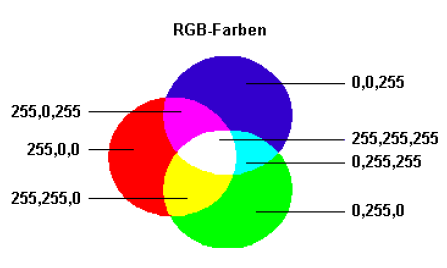
\includegraphics[width=0.8\textwidth]{img/rgb_farbmischung_steph.png}
	\caption[RGB-Farbmischung]{RGB-Farbmischung}
	\label{fig:farbmischung_steph}
\end{figure}


Im RGB-Farbmodell wird jede Farbe also durch ein Tripel aus den Grundfarben Rot, Grün und Blau beschrieben. Aus diesem Grund kann das RGB-Farbmodell als Farbwürfel dargestellt werden. Diesem Würfel liegt ein kartesisches Koordinatensystem zugrunde mit den 3 Achsen R; G; B. Innerhalb des Farbwürfels und an den begrenzenden Flächen ergeben sich alle erzeugbaren Farben. Diese Anzahl der Farben ist abhängig von den Intensitäten entlang der Achsen. Ist die Einstellung der Stärke der Beleuchtung in 256 Einheiten geteilt (numerisch also durch 1 Byte unterscheidbar), ergeben sich ${2}^8 * {2}^8 * {2}^8 = 16777216 $ mögliche Farbstufungen (entspricht einer Farbtiefe von 24 Byte).(s. Abbildung \ref{fig:farbwurfel_steph})

\begin{figure}[h]
	\centering
		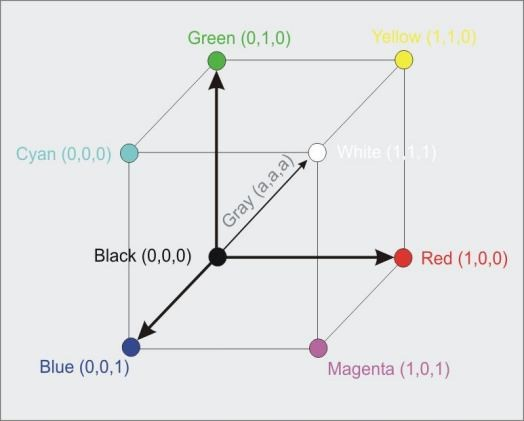
\includegraphics[width=0.6\textwidth]{img/rgb_farbwuerfel_steph.jpg}
	\caption[RGB-Farbwürfel(11)]{RGB-Farbwürfel(11)}
	\label{fig:farbwurfel_steph}
\end{figure}

Farben werden im RGB-Modell also als dreidimensionalen Vektorraum definiert. Die Vektoren dieses Raumes heißen Farbvalenzen, die Länge eines Vektors ist ein Maß für die Leuchtdichte und heißt Farbwert, seine Richtung bestimmt die Farbart. Die Basisvektoren heißen Primärvalenzen. Mit den Primärvalenzen R; G; B lässt sich also für jede Farbvalenz F eine Farbgleichung aufstellen:

\begin{center}
$ F = r * R +g * G + b * B $
\end{center}


Es sei hier erwähnt, dass es neben dem RGB-Farbmodell noch andere Modelle gibt. Diese werden hier nur genannt, da sie für die weitere Betrachtung keine Rolle spielen. Weitere Farbmodelle sind das CMY(K) - Farbmodell, HSV - Farbmodell, YUV - Farbmodell und das CIE XYZ – Farbmodell.
\subsection{\textbf{skalare Farbquantisierung}}
Bei skalaren Farbquantisierung wird jede der ursprünglichen Farbkomponenten C im Wertebereich [0...m-1] unabhängig von einander in den neuen Wertebereich [0...n-1] überführt, im einfachsten Fall durch eine lineare Quantisierung in der Form
\begin{center}
$ C' \leftarrow [C * \frac{n}{m}] $
\end{center}

für alle Farbkomponenten C. Ein Beispiel ist die Konvertierung eines Farbbilds mit 3 x 12-Bit-Komponenten, also 12 Bit pro Farbkanal mit m = 4096 möglichen Werten in ein herkömmliches RGB-Farbbild mit 3 x 8-Bit-Komponenten, also jeweils n = 256 Werten. Jeder Komponentenwert wird daher durch 4096/256 = 16 = $ 2^4 $ ganzzahlig dividiert oder, anders ausgedrückt, die untersten 4 Bits der zugehörigen Binärzahl werden einfach ignoriert. Abbildung 9 zeigt die skalare Quantisierung von Farbkomponenten durch Abtrennen niederwertiger Bits. Quantisierung von 3 x 12-Bit- auf 3 x 8-Bit-Farben. (s. Abbildung \ref{fig:rgb_farbbild_steph} RGB-Farbbild)

\begin{figure}[h]
	\centering
		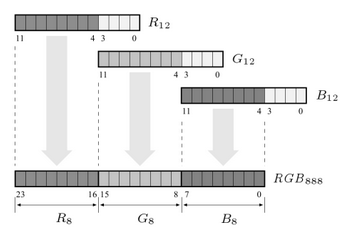
\includegraphics[width=0.6\textwidth]{img/rgb_farbbild_steph.png}
	\caption[RGB-Farbbild mit 3 x8-Bit-Komponenten (8)]{RGB-Farbbild mit 3 x8-Bit-Komponenten (8)}
\label{fig:rgb_farbbild_steph}
\end{figure}

Die skalare Quantisierung nimmt keine Rücksicht auf die Verteilung der Farben im ursprünglichen Bild. Sie wäre ideal, wenn die Farben im RGB-Würfel gleichverteilt sind. Bei natürlichen Bildern ist die Farbverteilung in der Regel jedoch ungleichförmig, sodass einzelne Regionen des Farbraums dicht besetzt sind, während andere Farben im Bild überhaupt nicht vorkommen. Der durch die skalare Quantisierung erzeugte Farbraum kann zwar auch die nicht vorhandenen Farben repräsentieren, dafür aber die Farben in dichteren Bereichen nicht fein genug abstufen. 
	

\subsection{\textbf{Zusammenfassung}}
Die Digitalisierung besteht aus Abtastung und Quantisierung. Durch die beschriebenen Eigenschaften der Abtastung und Quantisierung lässt sich also festhalten, dass ein digitales Bild immer nur eine Annäherung der Originalabbildung ist. Wir haben herausgestellt, die Abtastung ist die Aufteilung des Bildes in Bildpunkte (Pixel) und die Quantisierung die Bewertung der Helligkeit (Intensität) eines Pixels mittels einer festgelegten Grauwert- bzw. Farben-Menge, z.B. natürliche Zahlen von 0 bis 255. Die Qualität der Datenkompression eines digitalen Bildes hängt also maßgeblich von diesen beiden Faktoren ab. Wie wir herausgestellt haben ist die skalare Farbquantisierung ein einfaches und schnelles Verfahren, das den Bildinhalt selbst nicht berücksichtigt, zur Datenreduktion. Durch den zeitlich begrenzten Rahmen und Umfang dieser Arbeit in Hinsicht auf die Programmierung haben wir uns für die skalare Farbquantisierung entschieden, da die Vektorquantisierung maßgeblich von der Programmierung eines optimalen Codebuches abhängt. Ein zweiter Punkt für die skalare Quantisierung ist, dass in dieser Arbeit das Grundlegende Verständnis einer Quantisierung und deren Funktionsweise dargestellt werden soll.

\subsection{\textbf{Literaturverzeichnis}}

\begin{enumerate}
\item \textbf{Francis, Chukwumezie Millverton.} Vortragsskript der TU München. Proseminar : Grundlagen Bildverarbeitung/Bildverstehen Bildkompression. [PDF]. 21. 12 2005.
\item \textbf{www.mathemedien.de.} [Online] [Zitat vom: 28. 01 2016.] \url{http://www.mathemedien.de/datenkompression.html}

\item \textbf{Neumann} B. Bildverarbeitung für Einsteiger: Programmbeispiele mit Mathcad. s.l. : Springer Verlag, 2005.

\item \textbf{Tönnies, K.} Grundlagen der Bildverarbeitung. s.l. : Pearson Studium, 2005.

\item \textbf{Strutz, T.} Bilddatenkompression. s.l. : Vieweg+Teubner Verlag, 2005.

\item  \textbf{www.itwissen.info} [Online] [Zitat vom: 29. 01 2016.] \url{http://www.itwissen.info/definition/lexikon/Quantisierungsfehler-quatization-error.html.}

\item \textbf{www.itwissen.info} [Online] [Zitat vom: 29. 01 2016.] \url{http://www.itwissen.info/definition/lexikon/Abtastung-sampling.html>.}

\item \textbf{Burger, W. \& Burge} Digitale Bildverarbeitung: Eine algorithmische Einführung mit Java. s.l. : Springer Verlag, 2006.

\item \textbf{Ohm, J.}Digitale Bildcodierung: Repräsentation, Kompression und Übertragung von Bildsignalen . s.l. : Springer Verlag, 2013.

\item \textbf{Schmitz, R.} et al. Kompendium Medieninformatik: Mediennetze. s.l. : Springer Verlag, 2006.

\item \textbf{homepages.thm.} [Online] [Zitat vom: 01.02.2016.]\\
\url{https://homepages.thm.de/~hg10013/Lehre/MMS/SS01_WS0102/Farbmodelle/Kapitel/Kapitel4.html}
\end{enumerate}


\subsection{\textbf{Definitionen, Akronyme, Abkürzungen}}
\begin{acronym}[UV-Licht]
\acro{HfTL}{Hochschule für Telekommunikation Leipzig}
\acro{APP}{Kurzform für Applikation}
\acro{mbH}{mit beschränkter Haftung}
\acro{QIS}{Qualitätssteigerung der Hochschulverwaltung im Internet durch Selbstbedienung}
\acro{iCal}{Datenformat zum Austausch von Kalenderinhalten}
\acro{SoSe15}{Sommersemester 2015}
\acro{XML}{ Extensible Markup Language}
\acro{HTTPS}{HyperText Transfer Protocol Secure}
\acro{AES}{Advanced Encryption Standard}
\acro{SQL}{Structured Query Language}
\acro{.apk}{Android application package}
\acro{MTBF}{mean time between failure}
\acro{CI/CD}{Corperate Identity/Corperate Design}
\acro{GUI}{Graphical User Interface}
\acro{QuantiPig}{quantisiertes Picture}


\end{acronym}

\section{Vergleich der vorhandenen drei APPs}


Als Ausgangssituation wurden der Studentengruppe drei \acs{APP}s aus vorherigen Matrikeln vorgelegt, die ebenfalls Bilddaten komprimieren. Diese drei \acs{APP}s gilt es zu vergleichen und die Stärken herauszuarbeiten. Anhand dieser Ergebnisse gilt es eine neue \acs{APP} zu entwickeln.

\subsection{\textbf{Speicherplatzbedarf}}

Die Speicherbelastung wurde anhand folgender Aspekte betrachtet: 
\begin{itemize}
\item benötigter Speicherplatz der APP auf dem Smartphone
\item Speicherbelastung während des Betriebs
\end{itemize}

Während der Analyse wurde ein HTC One (M7), mit dem bereits die Testfotos gemacht wurden, verwendet. Die Ergebnisse werden in tabellarischer Form dargestellt und mit einer Einschätzung am Ende zusammengefasst.\\
\begin{figure}[h]
	\centering
		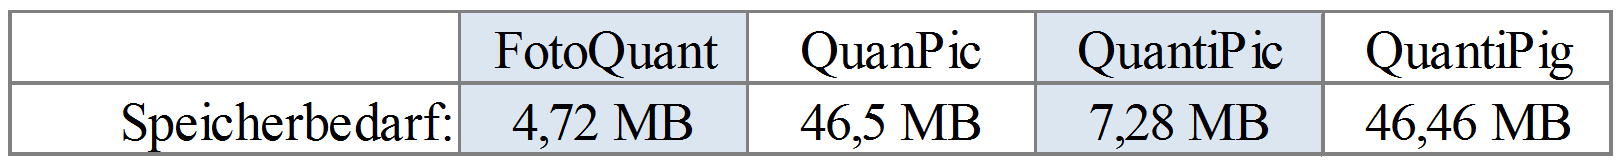
\includegraphics[width=0.8\textwidth]{img/speicherplatzbedarf_klein.png}
	\caption[Speicherplatzbedarf]{Speicherplatzbedarf}
	\label{fig:speicher_apps}
\end{figure}
\\\textbf{Einschätzung}\\

FotoQuant hat trotz seiner vielen Funktionen einen sehr geringen Speicherbedarf auf dem Smartphone. Nicht mal 5 MB werden in Anspruch genommen. Der Quellcode von 612 Zeilen länge (FotoQuantCameraView.java; FotoQuantCameraListener.java; FotoQuant.java) wird nur bedingt dafür verantwortlich sein. Auch QuantiPic belegt mit seinen drei Quantisierungsverfahren nur knappe 7,3 MB Speicher auf dem Testgerät. Der Quellcode ist hier mit 267 Zeilen wesentlich kompakter (MainActivity.java; + import von OpenCV Klassen), das zusätzliche Integrieren von einigen OpenCV Klassen erhöht dabei jedoch die Gesamtgröße. Beide APP‘s integrieren OpenCV nicht von vorn herein, es muss separat herunter geladen und installiert werden.
\\
Deutlich mehr Speicher belegt QuanPic. Mit fast 47 MB ist die Anwendungssoftware knapp zehn Mal größer als FotoQuant und das obwohl weniger Funktionen zur Verfügung stehen! Der Quellcode unterscheidet sich mit 696 Zeilen nur gering von den beiden Ersten APP‘s (MainActivity.java; NeueQuant.java). Der hohe Speicherplatzbedarf begründet sich allein durch das komplette Einbinden von OpenCV. 
\\
Aus den bestehenden APP‘s wurde QuanPic als Basis für QuantiPig gewählt. Erweitert um einige Vorteile aus FotoQuant und QuantiPic, teilt sich der Quellcode nun auf drei Hauptdateien. Mit 456 Zeilen (MainActivity.java; Pixel.java; Skalar.java) hat dieser die zweitkürzeste Länge. Kompakt und Funktional werden knapp 46,5 MB auf dem Testgerät belegt, denn auch hier ist OpenCV komplett integriert, so dass es keiner zusätzlichen Installation bedarf.

\subsection{\textbf{Speicherbelastung im Live-Betrieb}}

Die Analyse der Speicherbelastung erfolgte durch die Auswertung von Speicher- und CPU-Auslastung während des Live-Betriebs. Dabei wurde unter anderem die APP „System Monitor“ auf dem Testgerät installiert und die Speicherbelastung aufgezeichnet. Als Testumgebung wurde vor jeder Aufzeichnung sichergestellt, dass nur die zu testende App sowie „System Monitor“ aktiv geöffnet waren. Während der Aufzeichnung wurden die einzelnen Modi der APP‘s durchgetestet. Eine Aufzeichnung war nicht länger als 3 Minuten, wobei alle 1000 ms der Speicherbedarf durch „System Monitor“ ausgelesen wurde. Die erfassten Werte wurden im Mittelwert zusammengefasst und werden nun tabellarisch aufgelistet. Die Rohdaten befinden sich im Anhang „Analyseergebnisse durch System Monitor“.  (siehe \ref{ssec:analyse})

\begin{figure}[h]
	\centering
		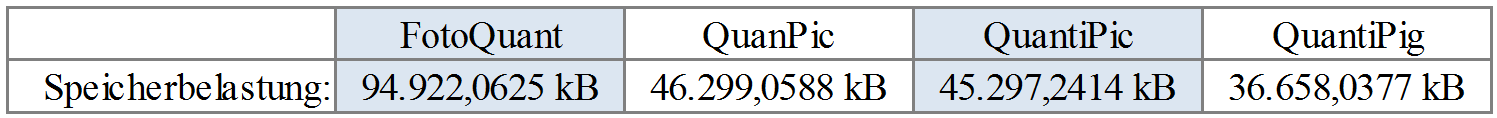
\includegraphics[width=1.0\textwidth]{img/speicherbelastung_klein.png}
	\caption[Speicherbelastung durch System Monitor]{Speicherbelastung}
	\label{fig:speicherbel_apps}
\end{figure}

Eine zweite Möglichkeit die Speicherbelastung zu ermitteln erfolgte durch den „Memory Monitor“ und „CPU Monitor“ von Android Studio. Zur Vorbereitung wurde die entsprechende APP in Android Studio, sowie auf dem Testgerät gestartet. Das Monitoring ermöglicht eine grafische Auswertung der folgenden Punkte:

\begin{itemize}
\item Total Memory, allocted Memory, Free Memory
\item Total CPU Usage, User Usage, Kernel Usage
\end{itemize}

Für die Analyse wurde die Belastung jeweils zum APP-Start, während der Modi sowie zum Beenden betrachtet. Die ermittelten Werte wurden wieder im Mittelwert zusammengefasst (s. Abbildung \ref{fig:speicherbel2_apps})\\\

\begin{figure}[h]
	\centering
		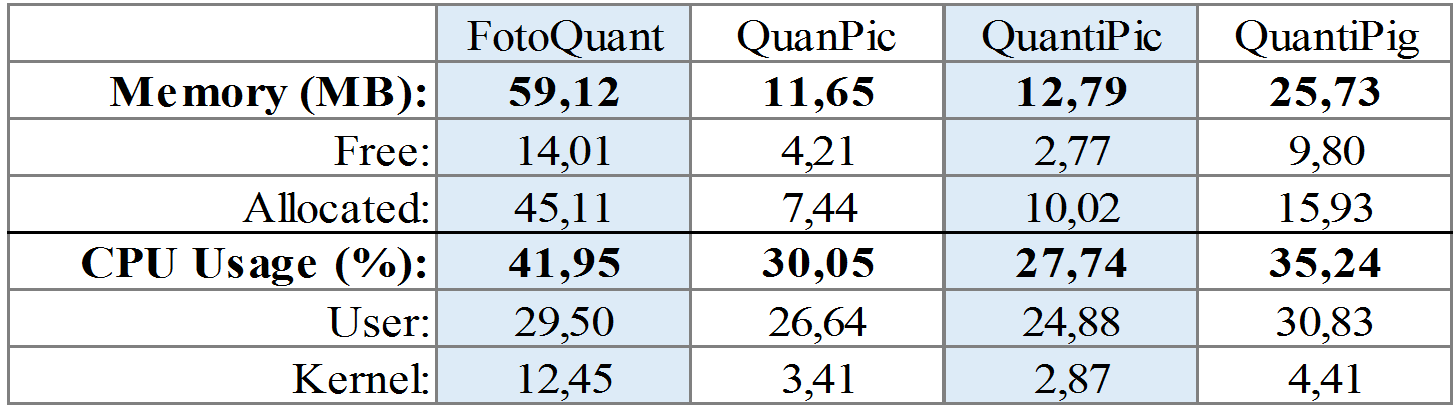
\includegraphics[width=0.8\textwidth]{img/speicherbelastung_gross.png}
	\caption[Speicherbelastung durch Memory/- und CPU-Monitor]{Speicherbelastung durch Memory/- und CPU-Monitor}
	\label{fig:speicherbel2_apps}
\end{figure} 

\textbf{Einschätzung}
\\
\\
Beide Vorgehen machen deutlich, dass zwei APP’s eine sehr geringe Speicherbelastung haben, während zwei APP’s einen wesentlich höheren Anspruch besitzen. FotoQuant kann seinen Vorteil aus dem geringen Speicherplatzbedarf nicht durch eine geringe Speicherbelastung erweitern. Im Gegenteil, die APP ist in der Performance durch den fast dauerhaften Anspruch auf 45 MB Speicher und knapp 42\% CPU-Leistung sehr langsam. QuantiPig dagegen, welches auf QuanPic aufbaut, hat zwar ebenfalls einen hohen Anspruch auf Speicher und CPU, kann die Performance aber deutlich steigern und erreicht mit knapp 26 MB Speicheranspruch eine geringere Belastung des Testgerätes. 
Wesentlich effizienter kommen in beiden Tests die APP QuanPic und QuantiPic davon. QuanPic hat trotz seines Speicherplatzbedarfs eine sehr geringe Speicher- und CPU-Belastung. Im Schnitt benötigt es gerade mal 7,44 MB Speicher und belastet den CPU dabei mit nur 30\%. Die Performance ist dadurch sehr gut und ermöglicht ein ruckelfreies arbeiten mit der App. Auch QuantiPic hat mit durchschnittlich 10 MB Speicherbelastung einen sehr geringen Anspruch an das Testgerät. Die CPU-Belastung ist dabei noch etwas kleiner gegenüber QuanPic. Mit knapp 27,8\% lässt sich die APP sehr flüssig bedienen und das trotz des größeren Funktionsumfangs.
Eine Übersicht über die Ergebnisse des Memory- und CPU-Monitors sehen Sie in Abbildung \ref{fig:analyseergebnisse_maik}.

\begin{figure}
	\centering
		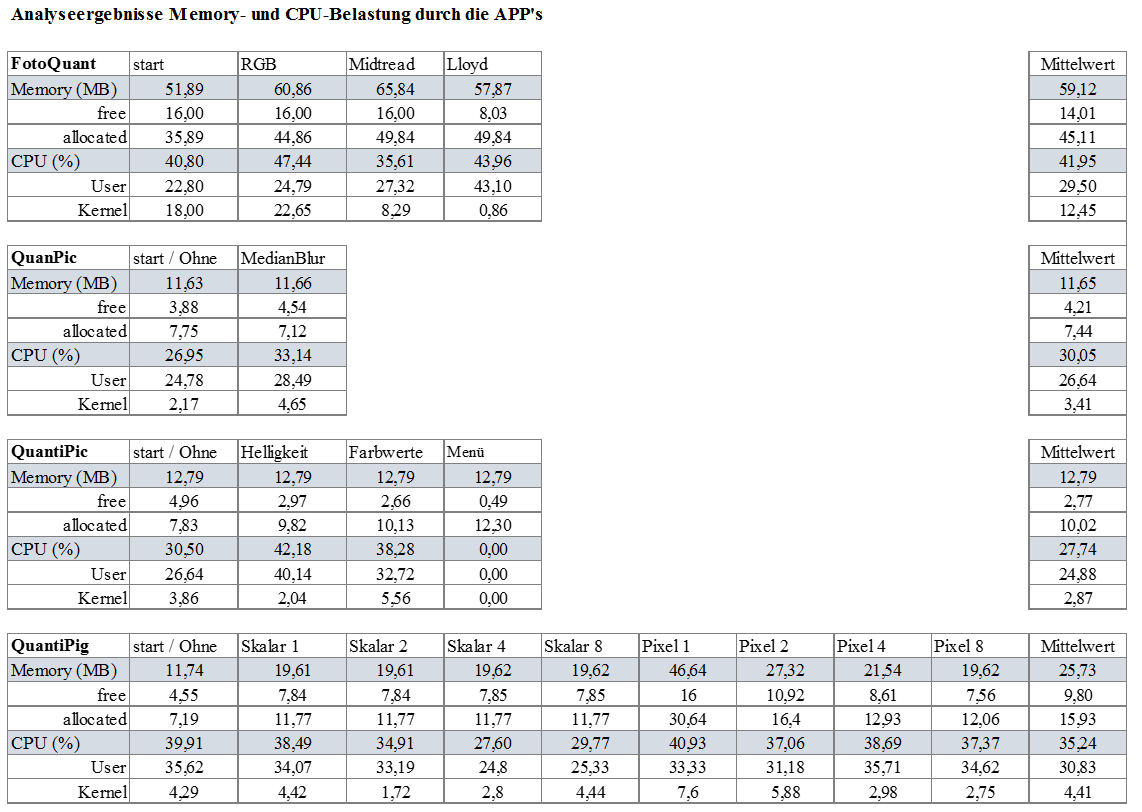
\includegraphics[width=1.0\textwidth]{img/analyseergebnisse_maik.png}
	\caption[ Ergebnisse AndroidStudio Memory- und CPU-Monitor]{ Ergebnisse AndroidStudio Memory- und CPU-Monitor}
	\label{fig:analyseergebnisse_maik}
\end{figure} 




\subsection{\textbf{Vergleich der vorhandenen drei \acs{APP}s}}
\begin{landscape}

\newpage

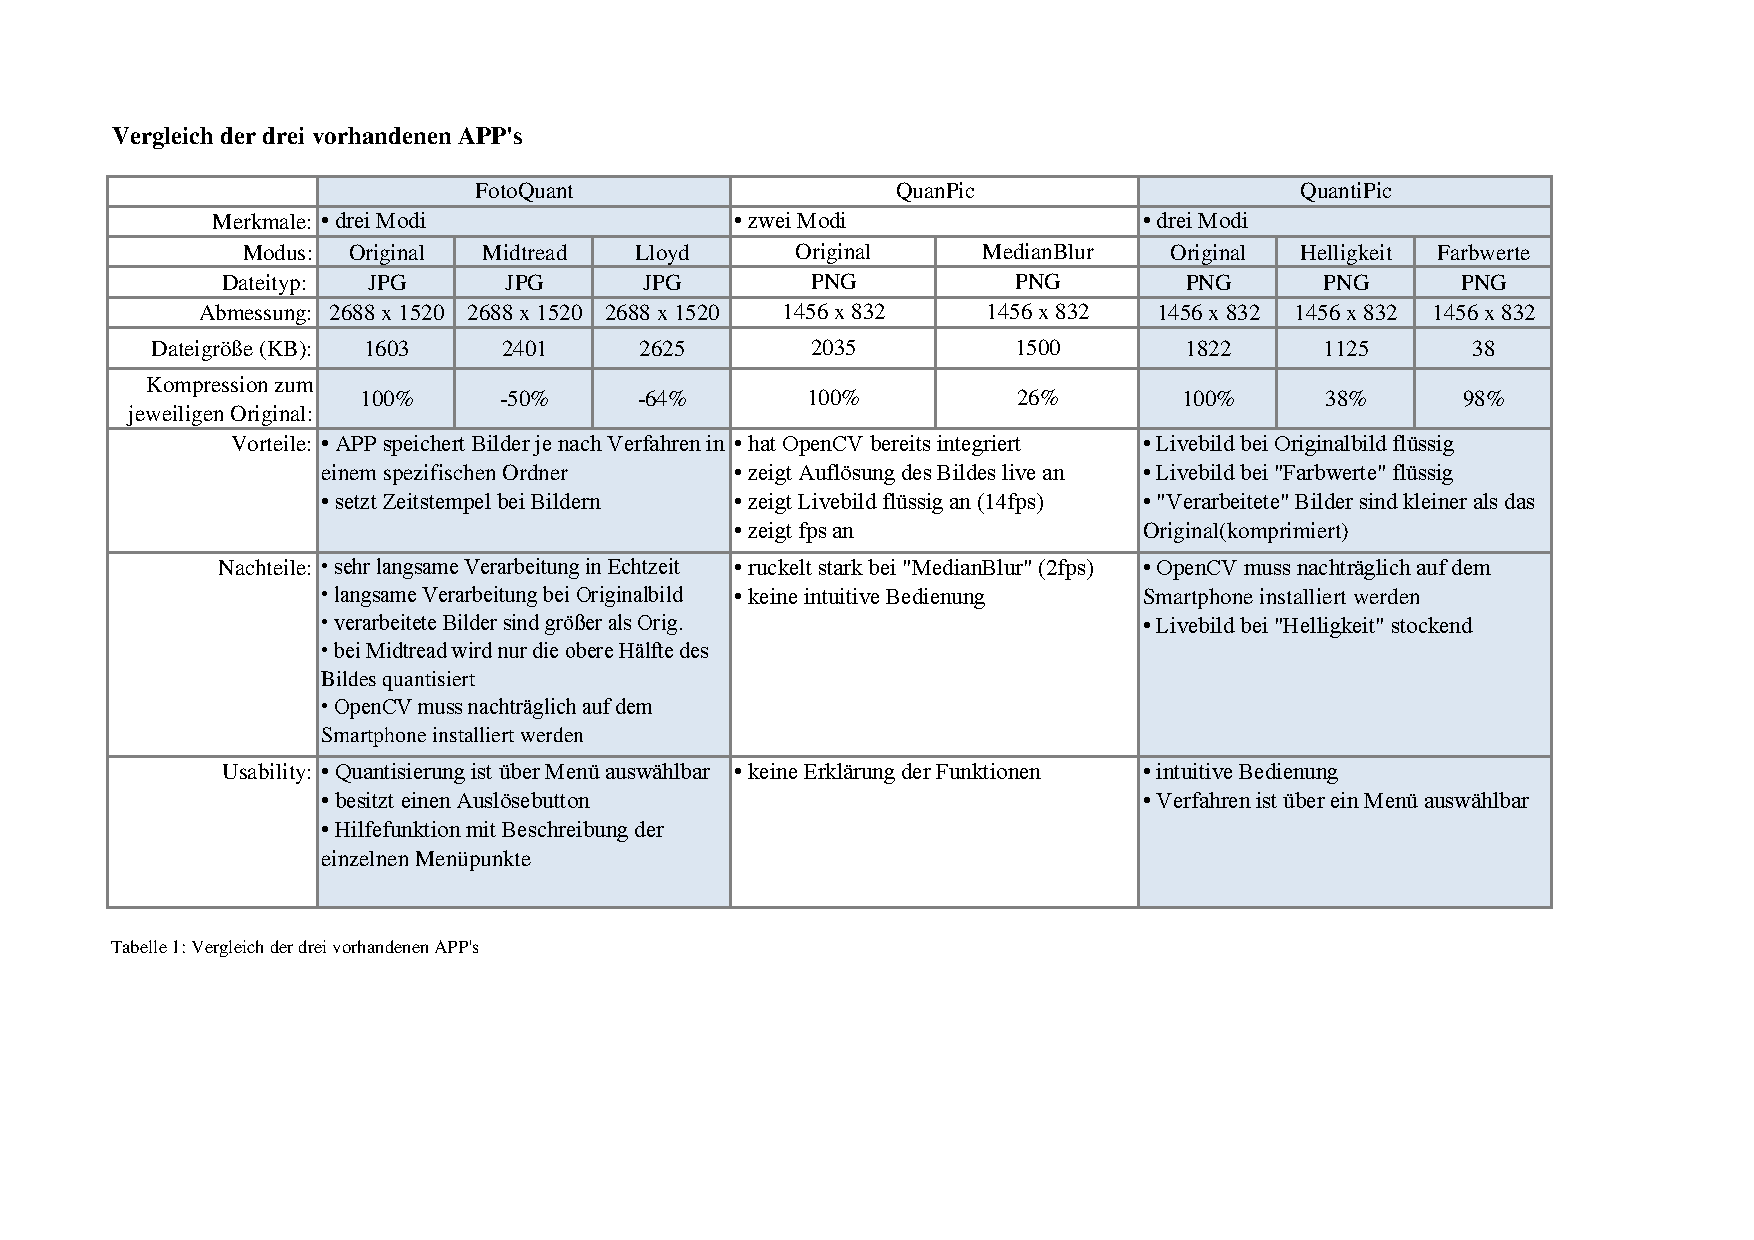
\includepdf[landscape=true,pages=-]{04_Anhang/files/Vergleich_Apps.pdf}


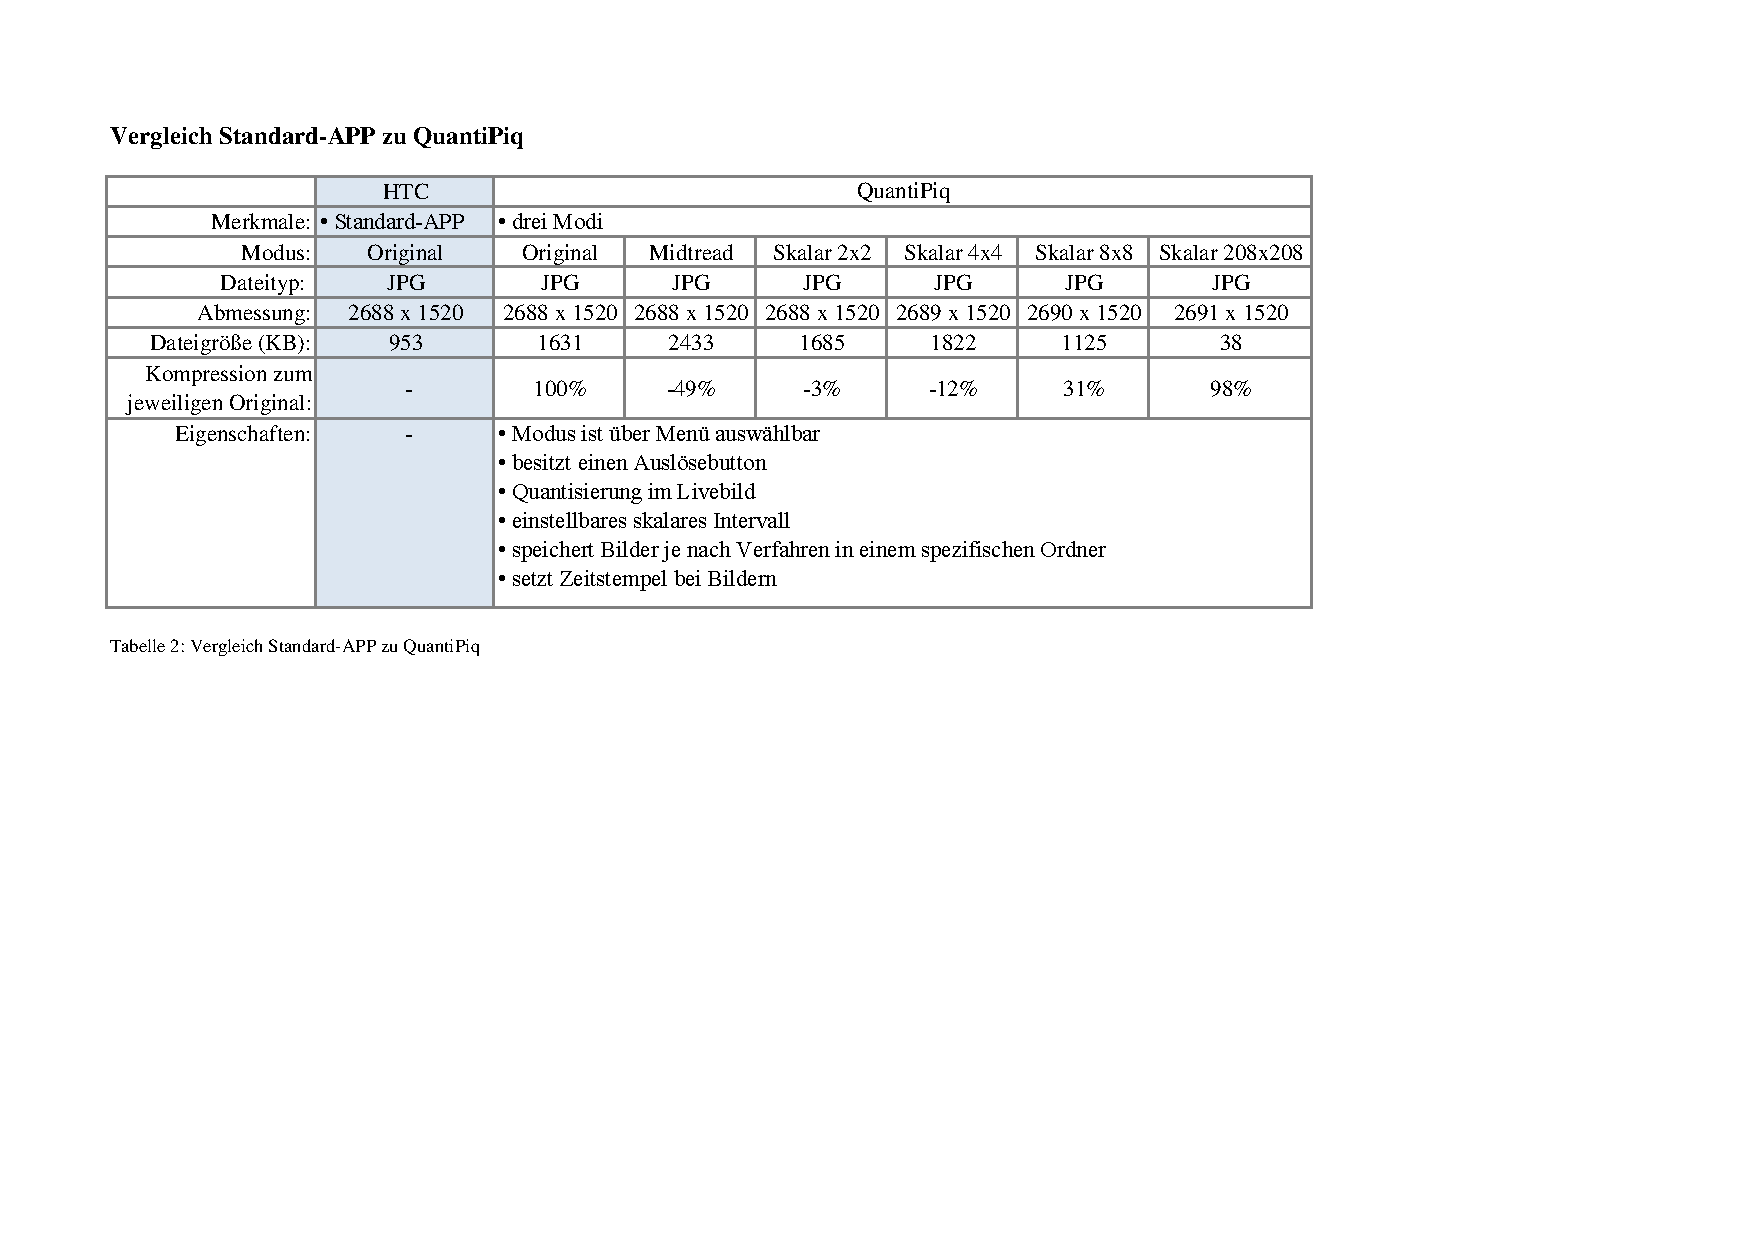
\includepdf[landscape=true,pages=-,noautoscale]{04_Anhang/files/Vergleich2.pdf}

\end{landscape}


\subsection{\textbf{Beispielbilder}}

\begin{landscape}

\begin{figure}[h]
	\centering
		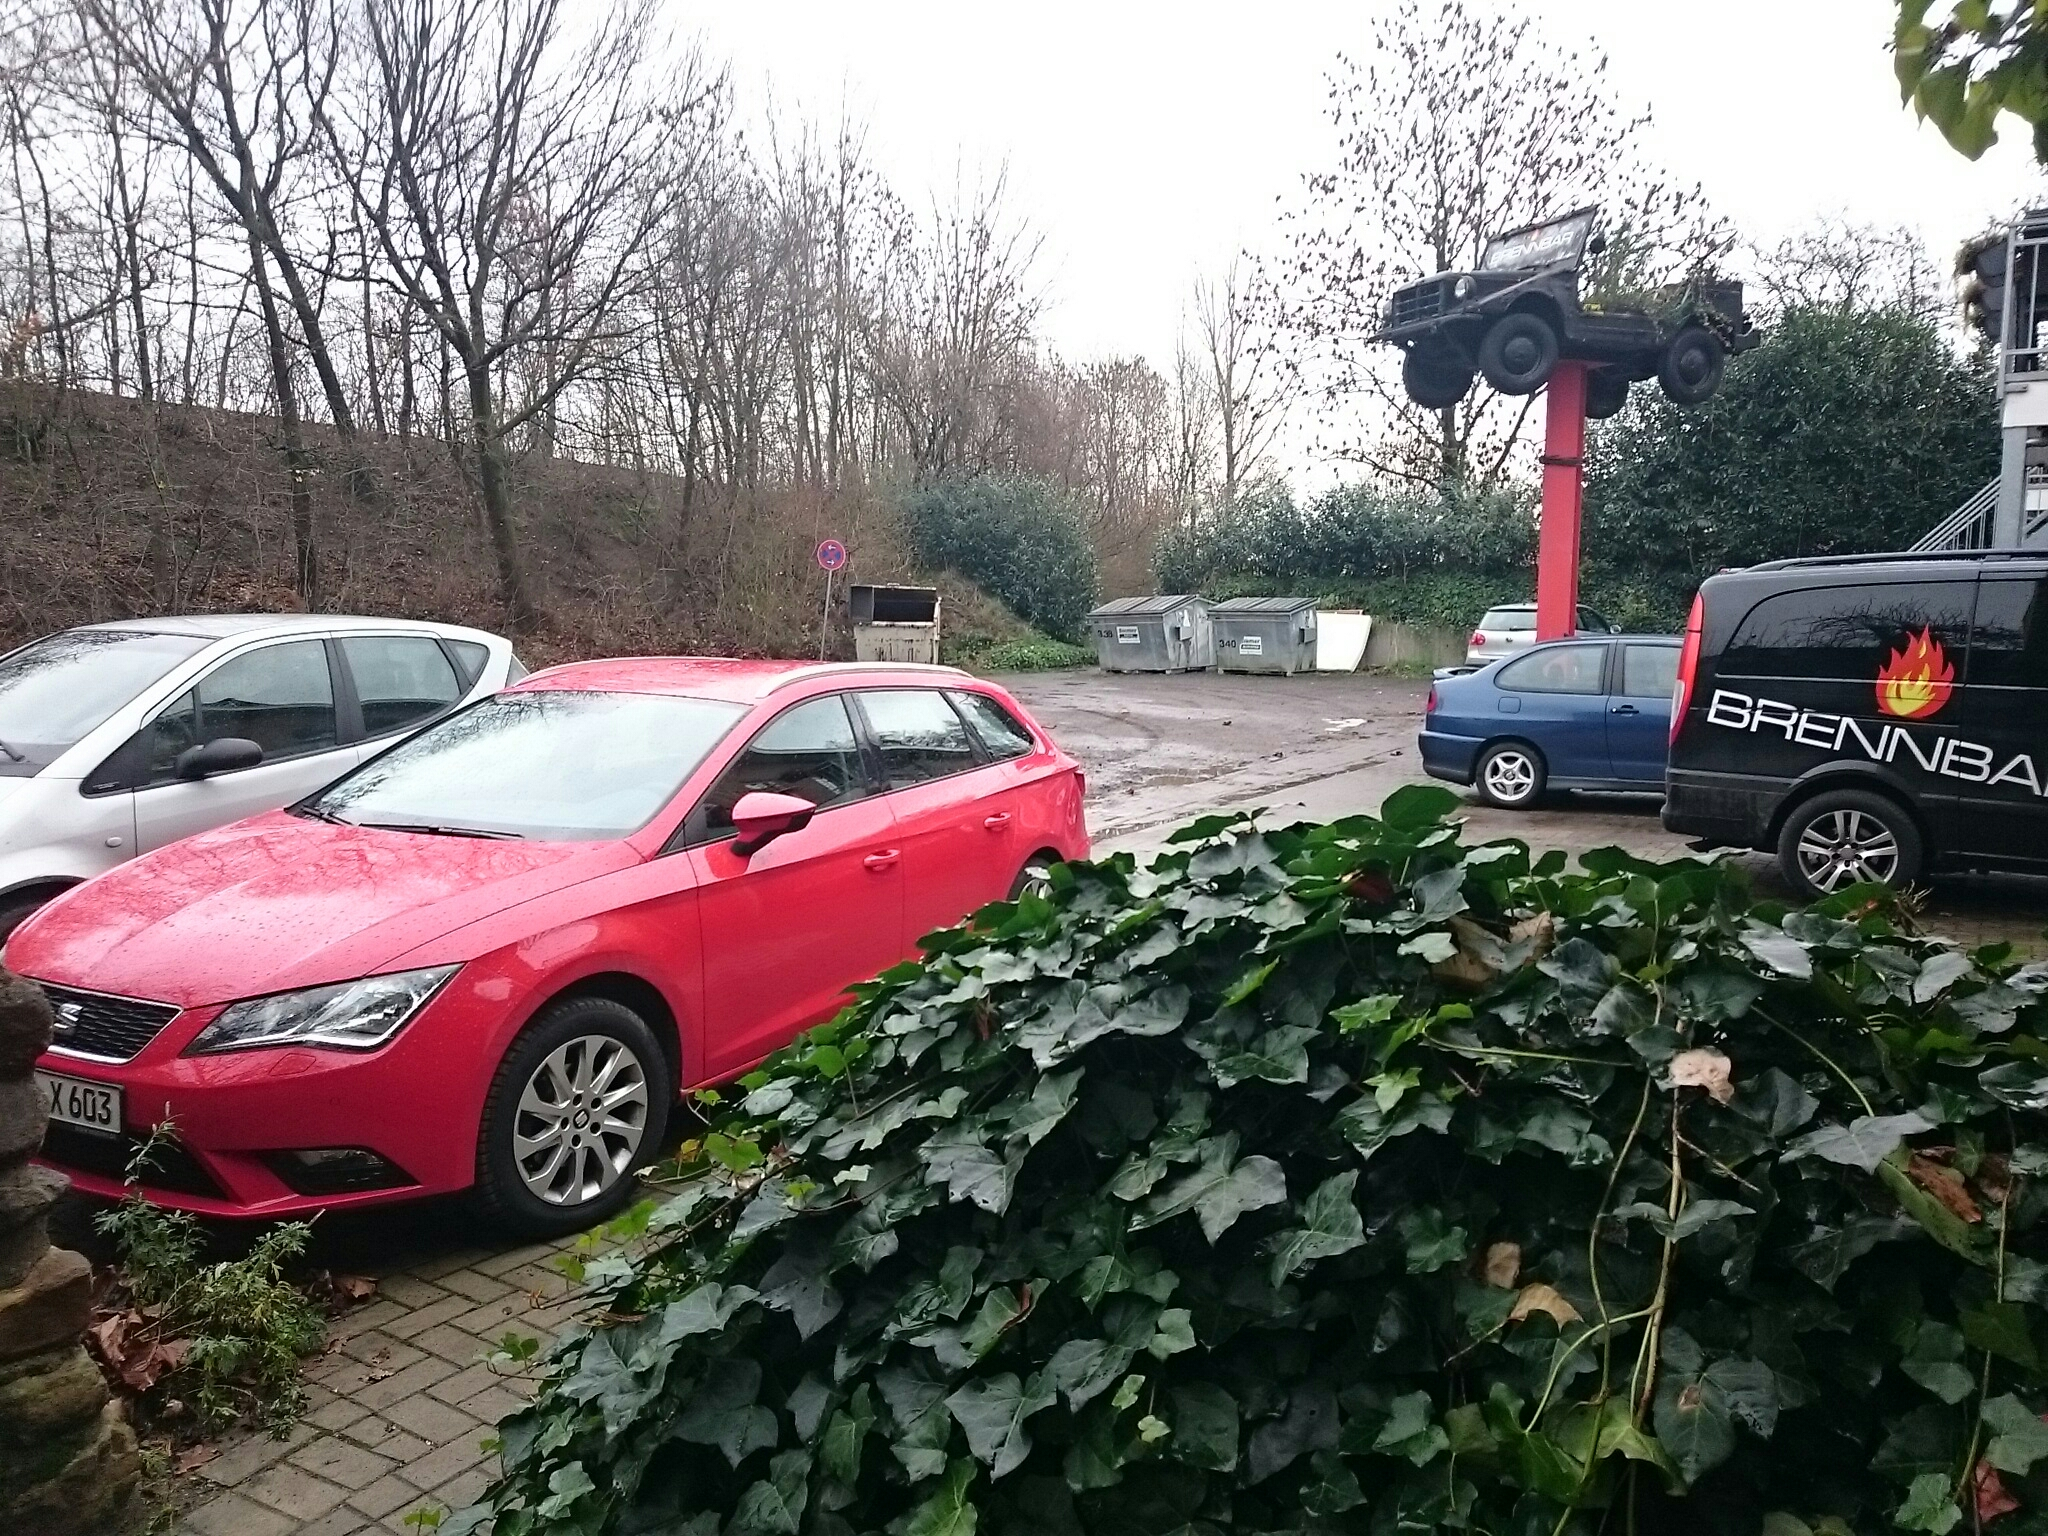
\includegraphics[width=1.4\textwidth]{img/Fotos/FotoQuant_Original.jpg}
	\caption[FotoQuant Original]{FotoQuant Originalbild}
	\label{fig:quant_ori}
\end{figure}

\begin{figure}[h]
	\label{fig:quant_mid}
	\centering
		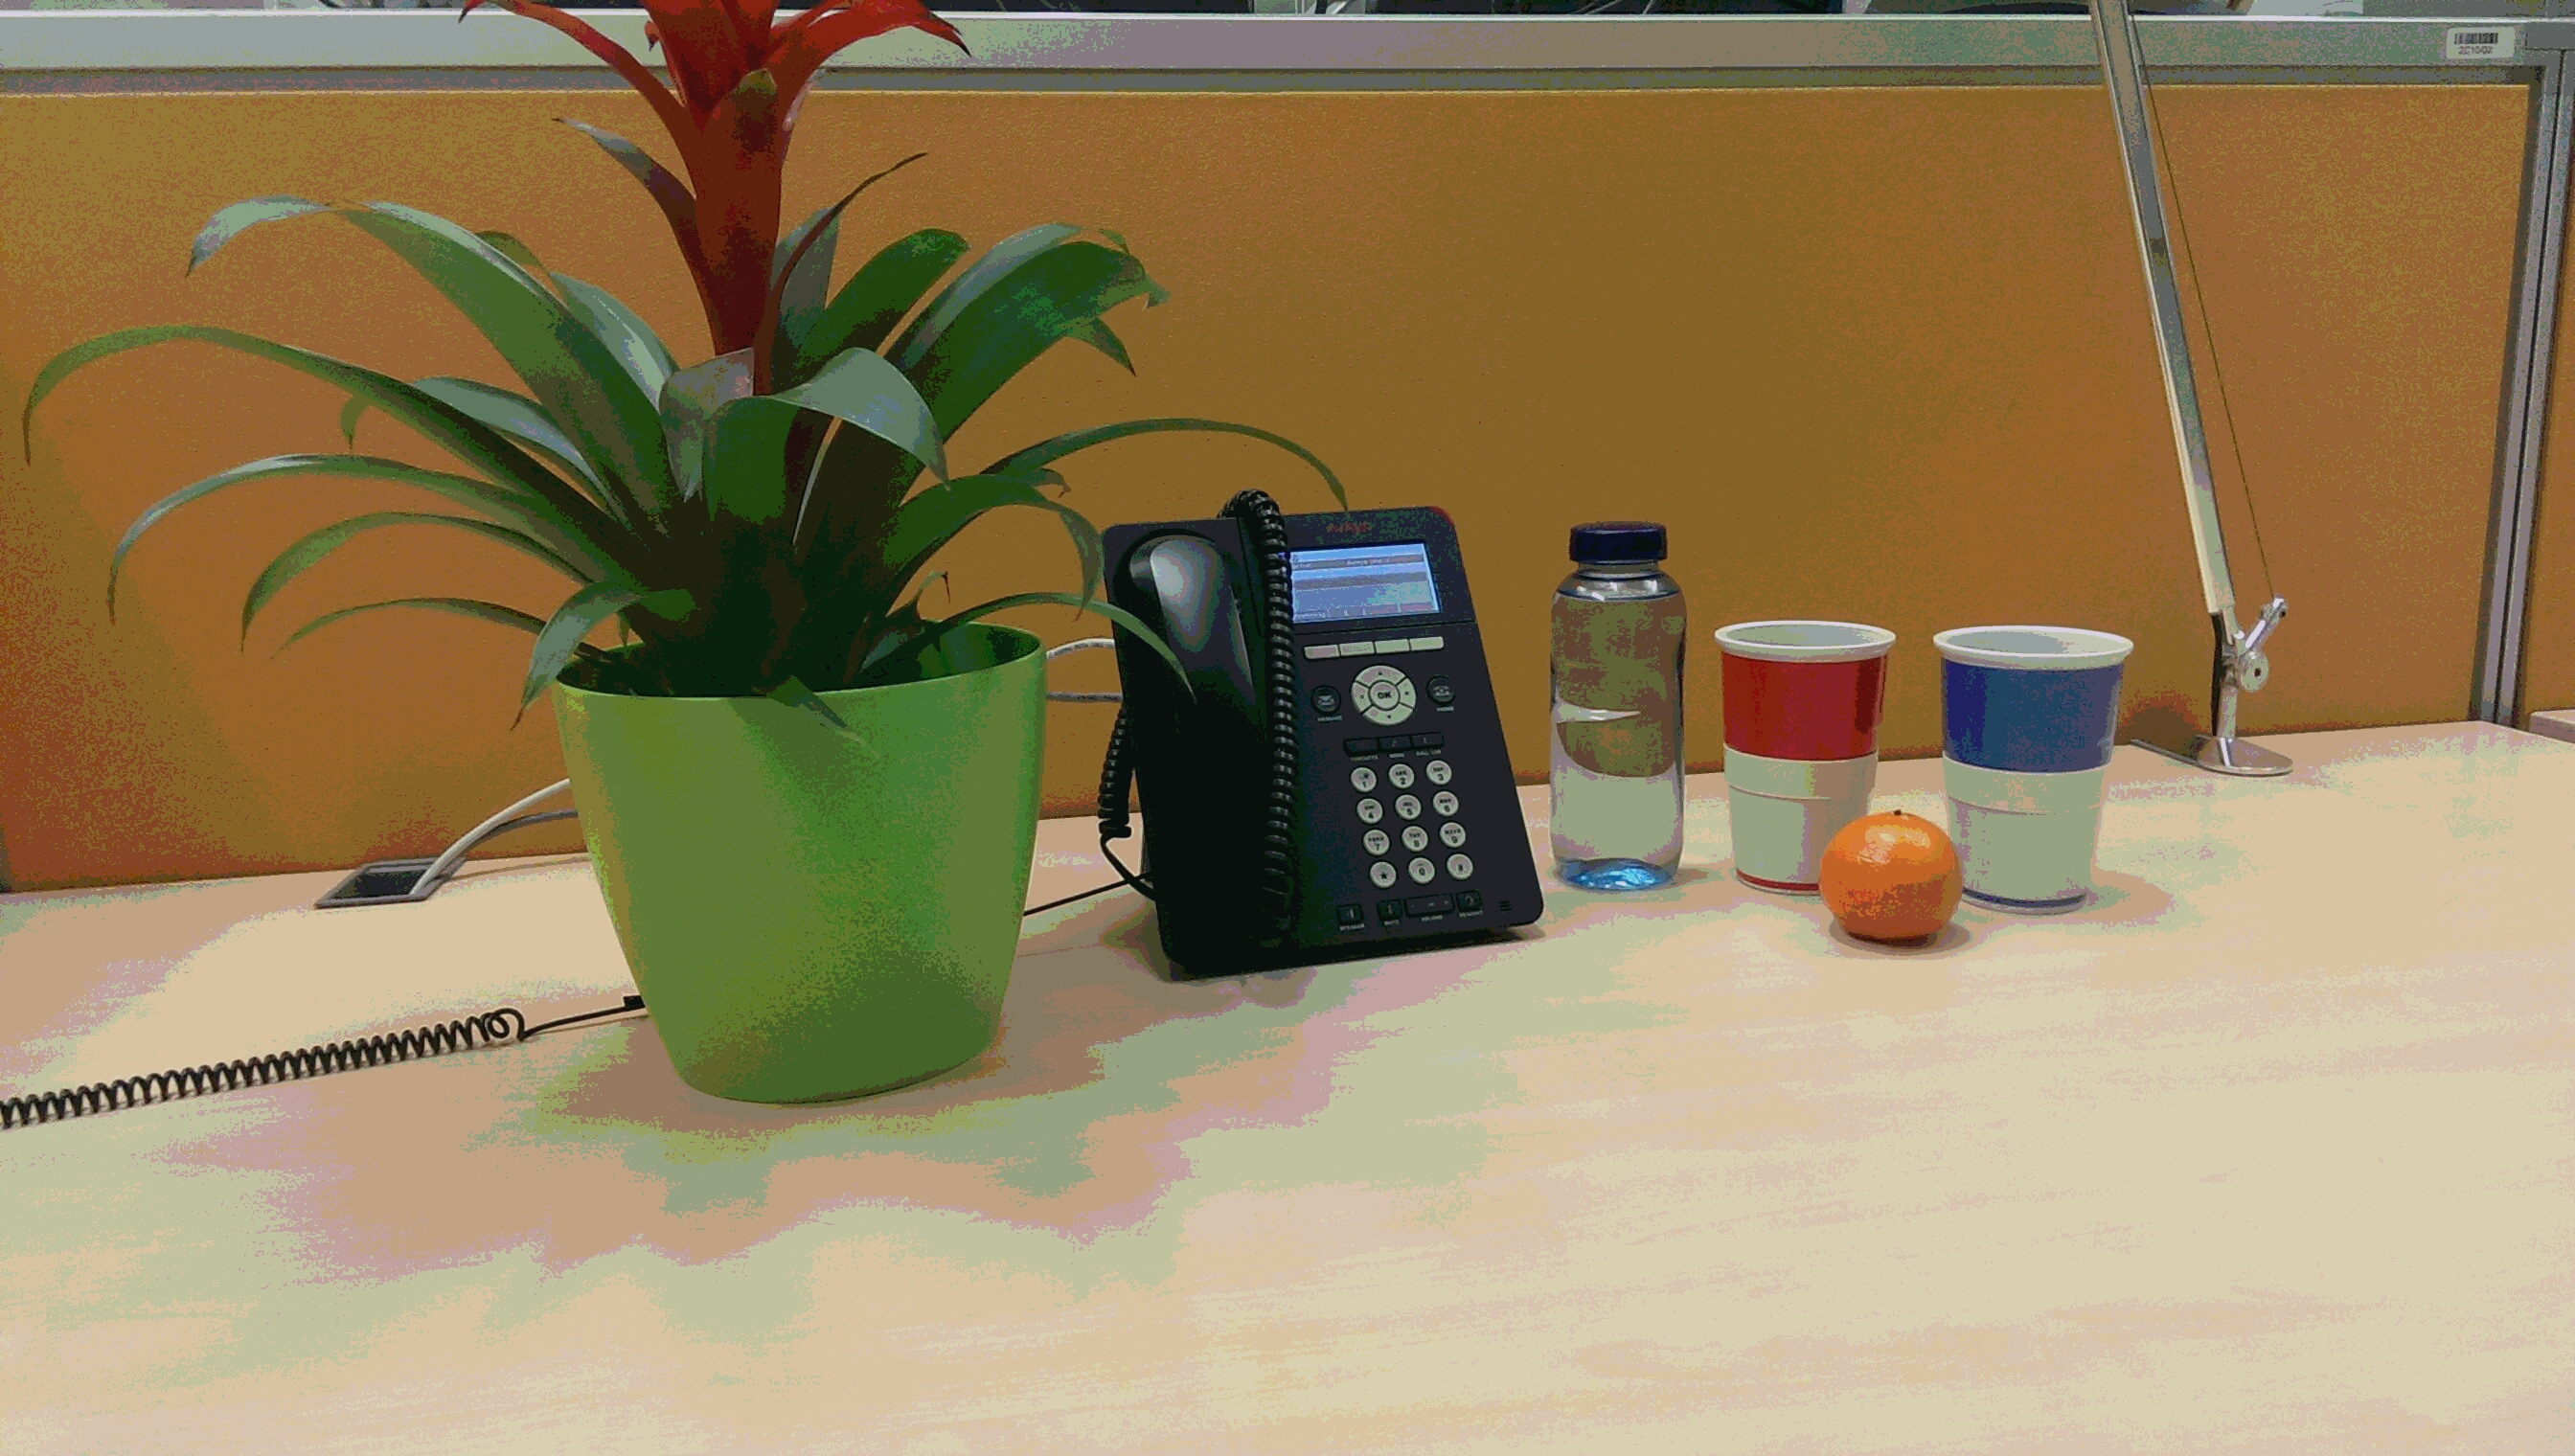
\includegraphics[width=1.4\textwidth]{img/Fotos/FotoQuant_Lloyd.jpg}
	\caption[FotoQuant Lloyd]{FotoQuant Lloyd-Modus}
	\label{fig:quant_lloyd}
\end{figure}

\begin{figure}[h]
	\centering
		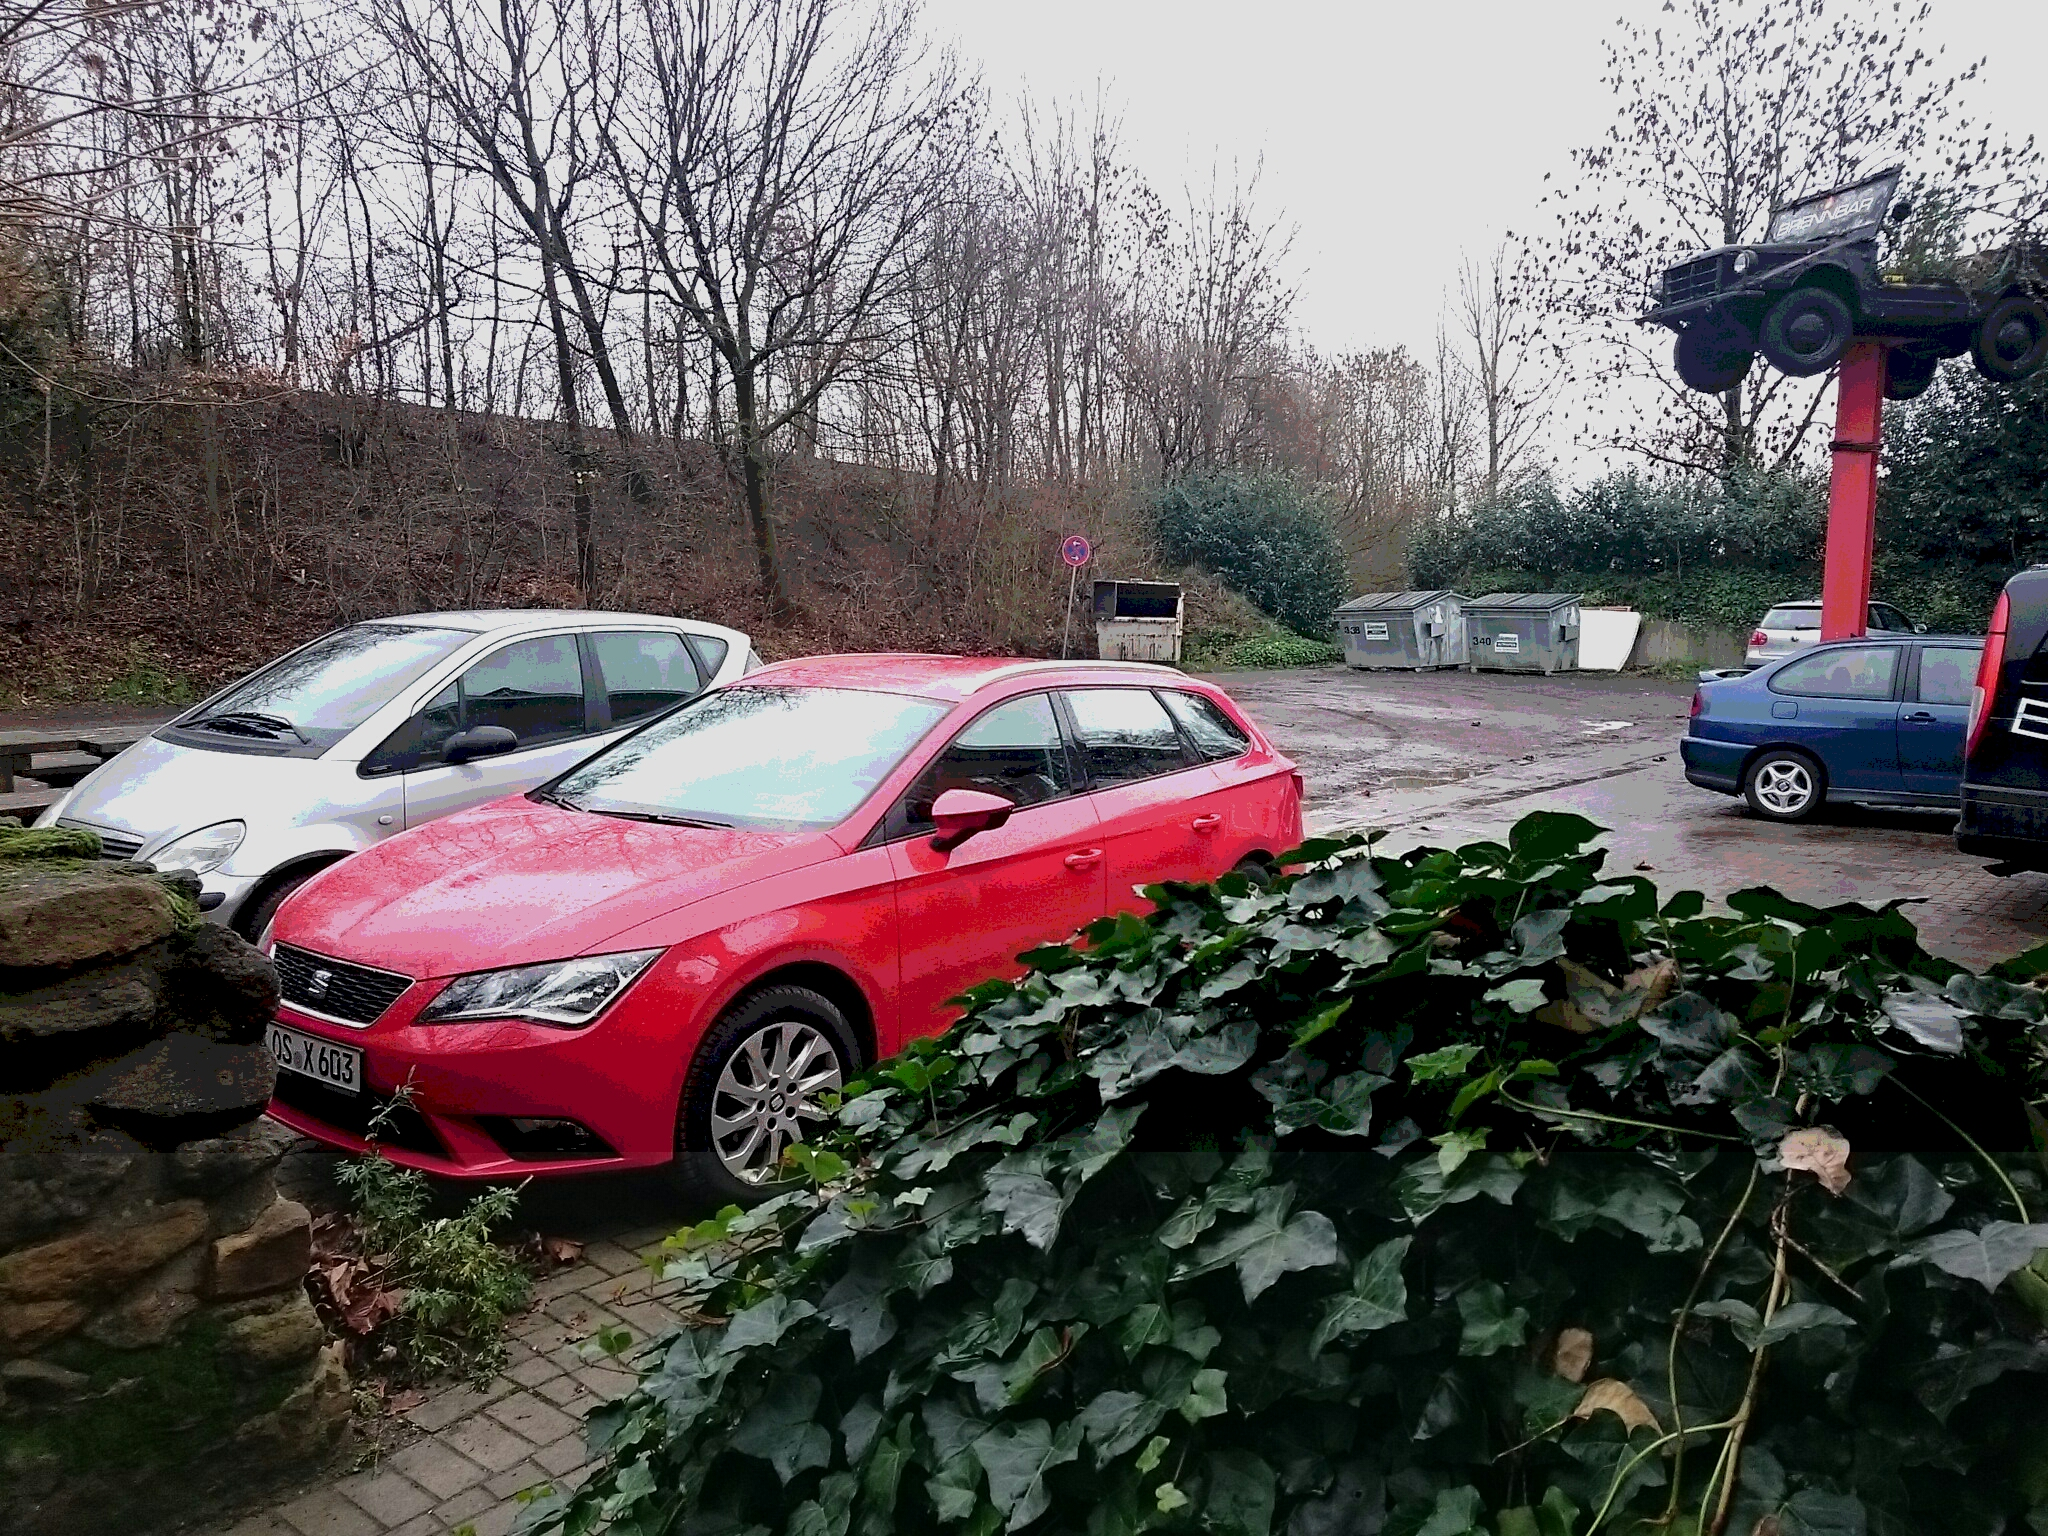
\includegraphics[width=1.4\textwidth]{img/Fotos/FotoQuant_Midtread.jpg}
	\caption[FotoQuant MidTread]{FotoQuant MidTread-Modus}
	\label{fig:quant_mid}
\end{figure}

\begin{figure}[h]
	\centering
		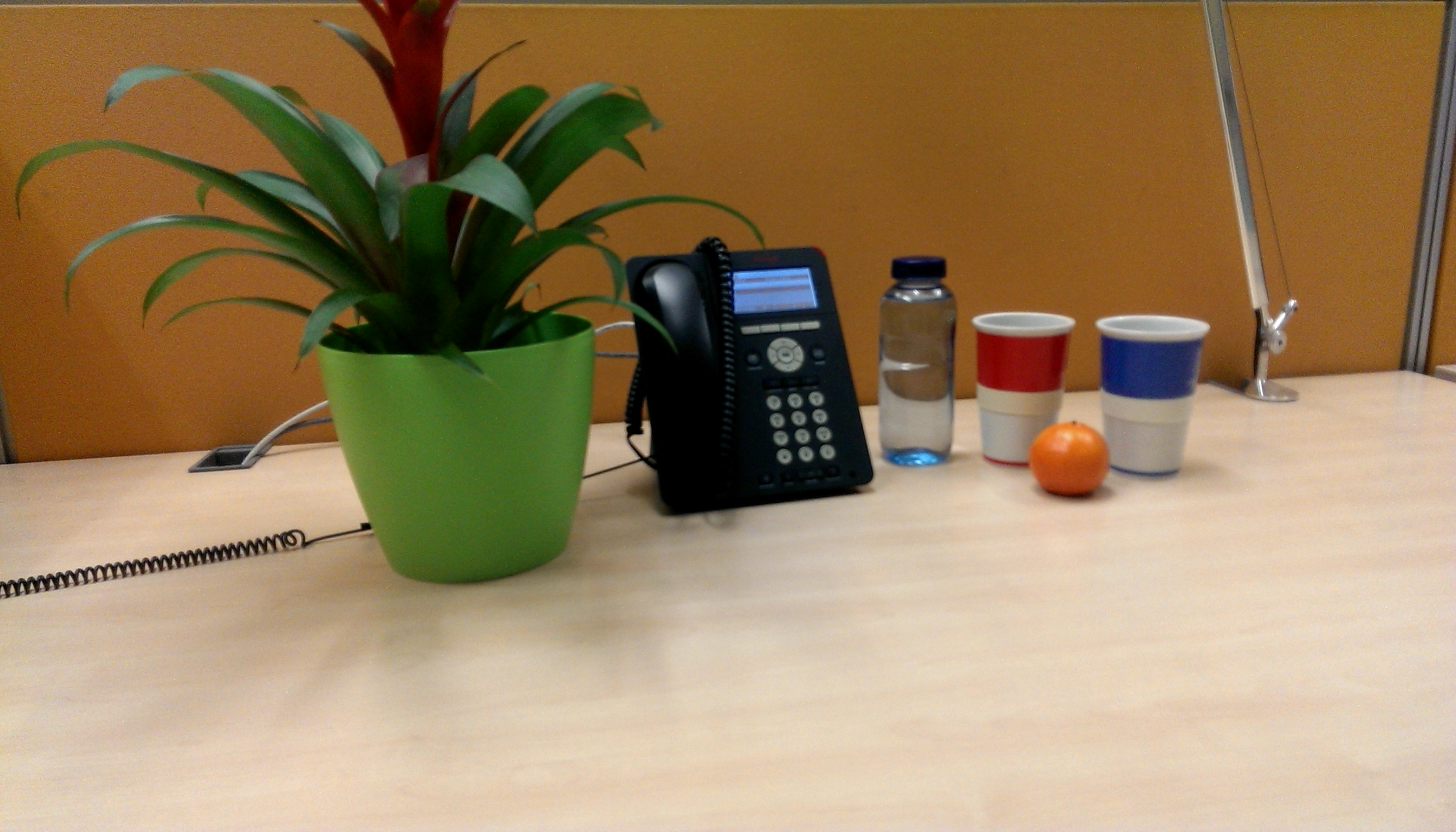
\includegraphics[width=1.4\textwidth]{img/Fotos/QuanPic_Original.png}
	\caption[QuanPic Original]{Quanpic im Originalbild-Modus}
	\label{fig:quan_orig}
\end{figure}

\begin{figure}[h]
	\centering
		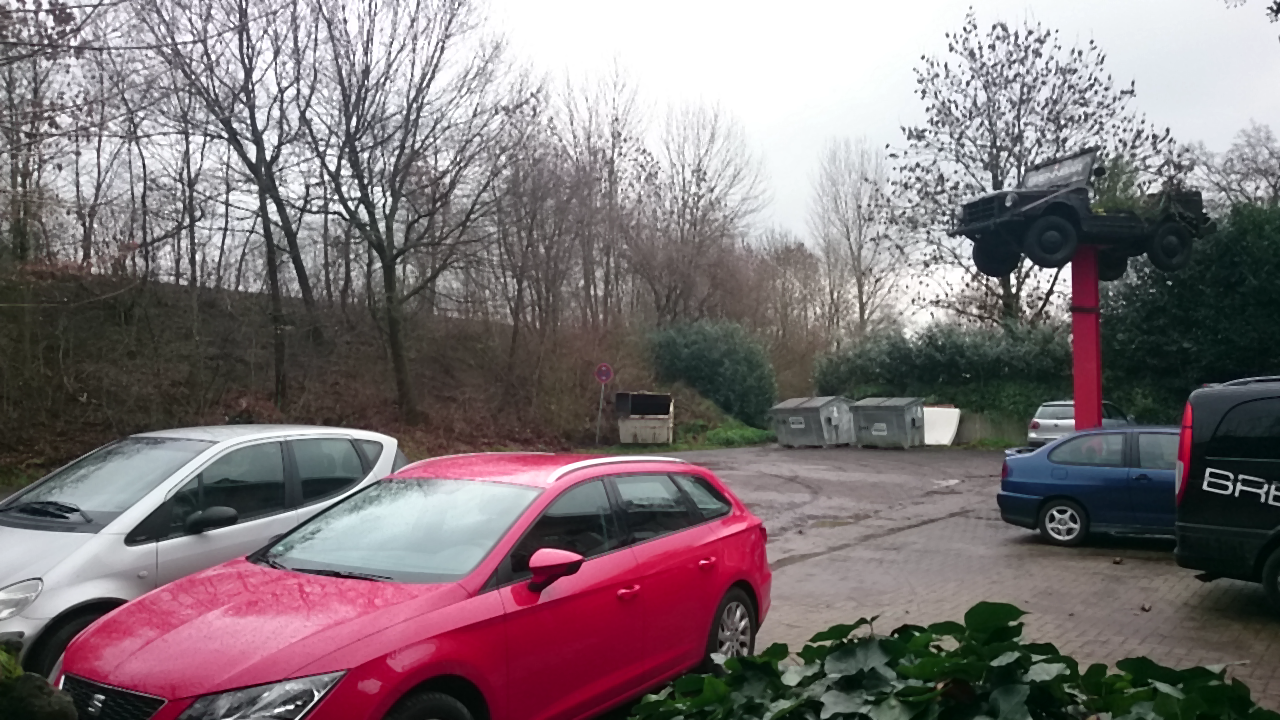
\includegraphics[width=1.4\textwidth]{img/Fotos/QuanPic_Medianblur.png}
	\caption[QuanPic MedianBlur]{Quanpic im MedianBlur-Modus}
	\label{fig:quan_med}
\end{figure}

\begin{figure}[h]
	\centering
		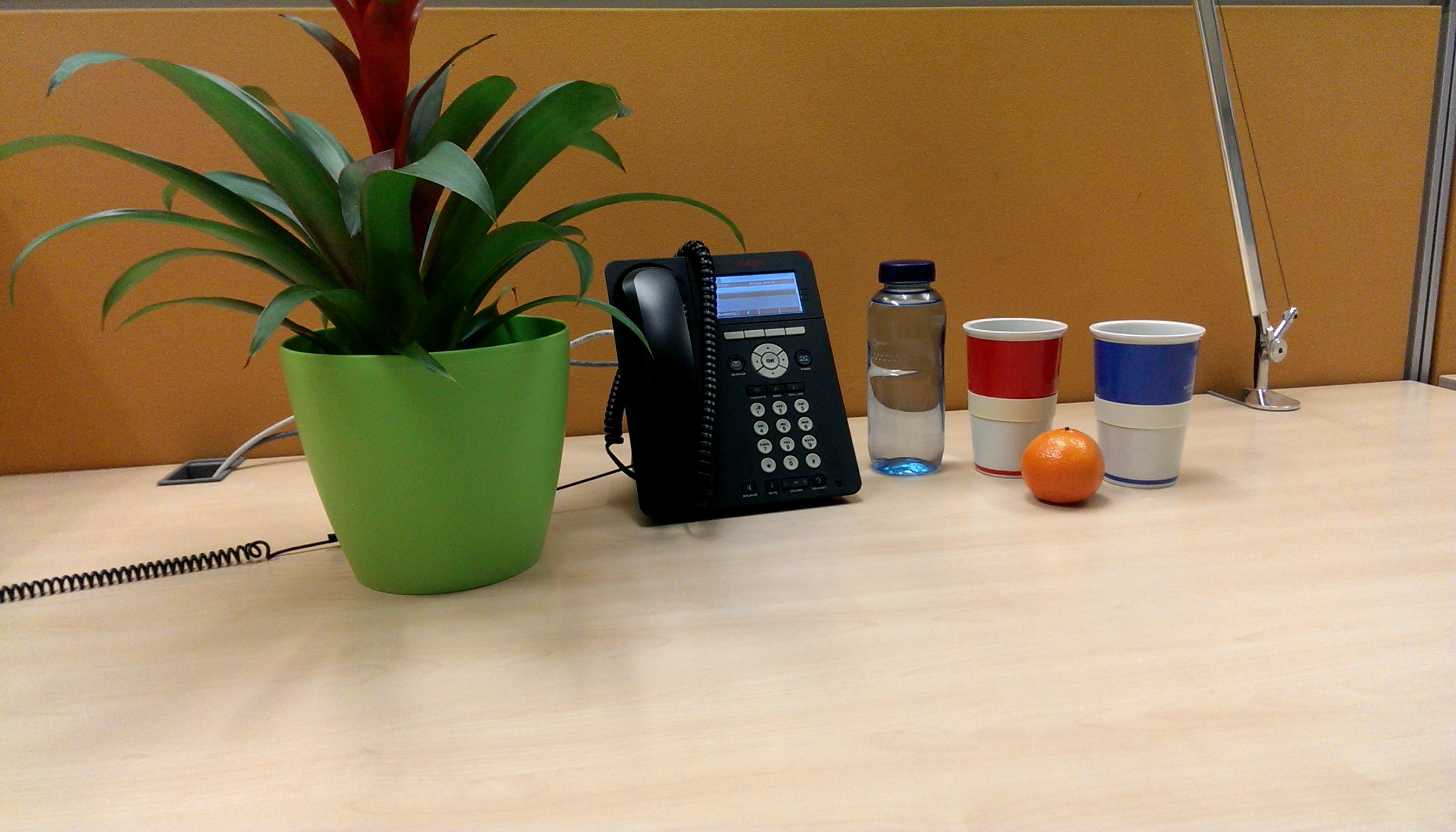
\includegraphics[width=1.4\textwidth]{img/Fotos/QuantiPic_Original.png}
	\caption[QuantiPic Originalbild]{QuantiPic im Originalbild-Modus}
	\label{fig:quanti_orig}
\end{figure}

\begin{figure}[h]
	\centering
		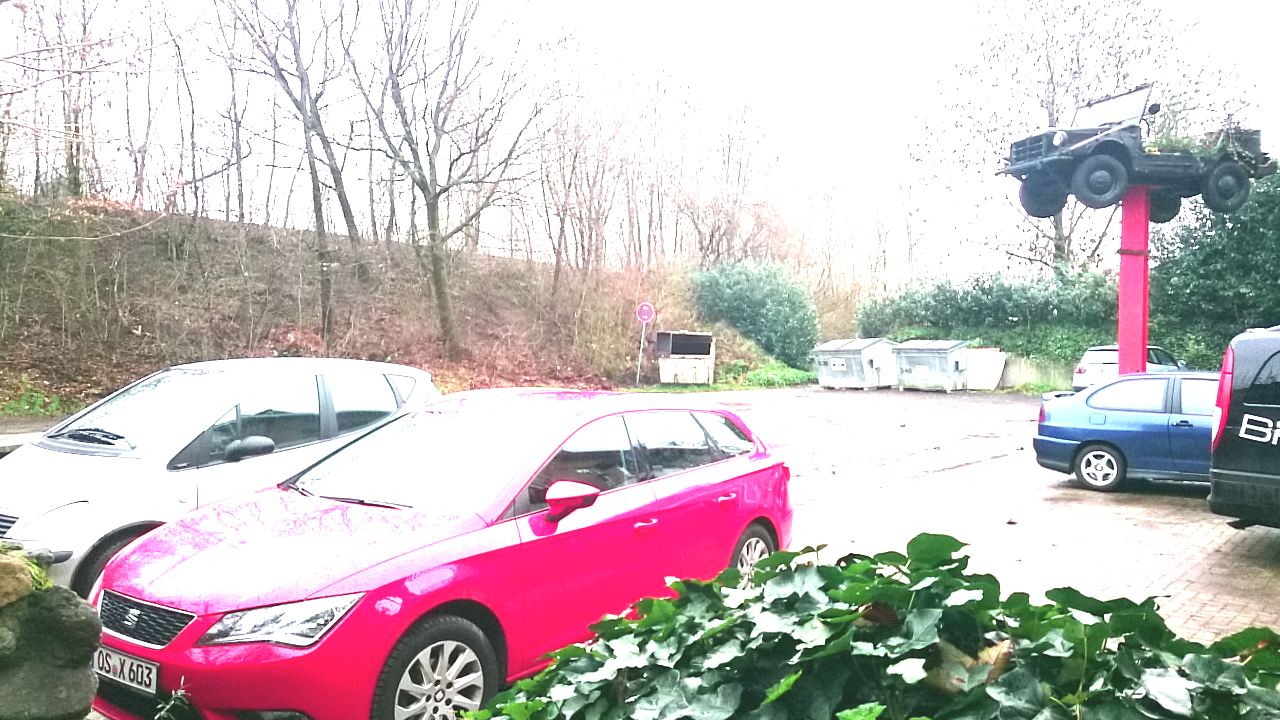
\includegraphics[width=1.4\textwidth]{img/Fotos/QuantiPic_Helligkeit.png}
	\caption[QuantiPic Helligkeit]{QuantiPic im Helligkeits-Modus}
	\label{fig:quanti_hell}
\end{figure}

\begin{figure}[h]
	\centering
		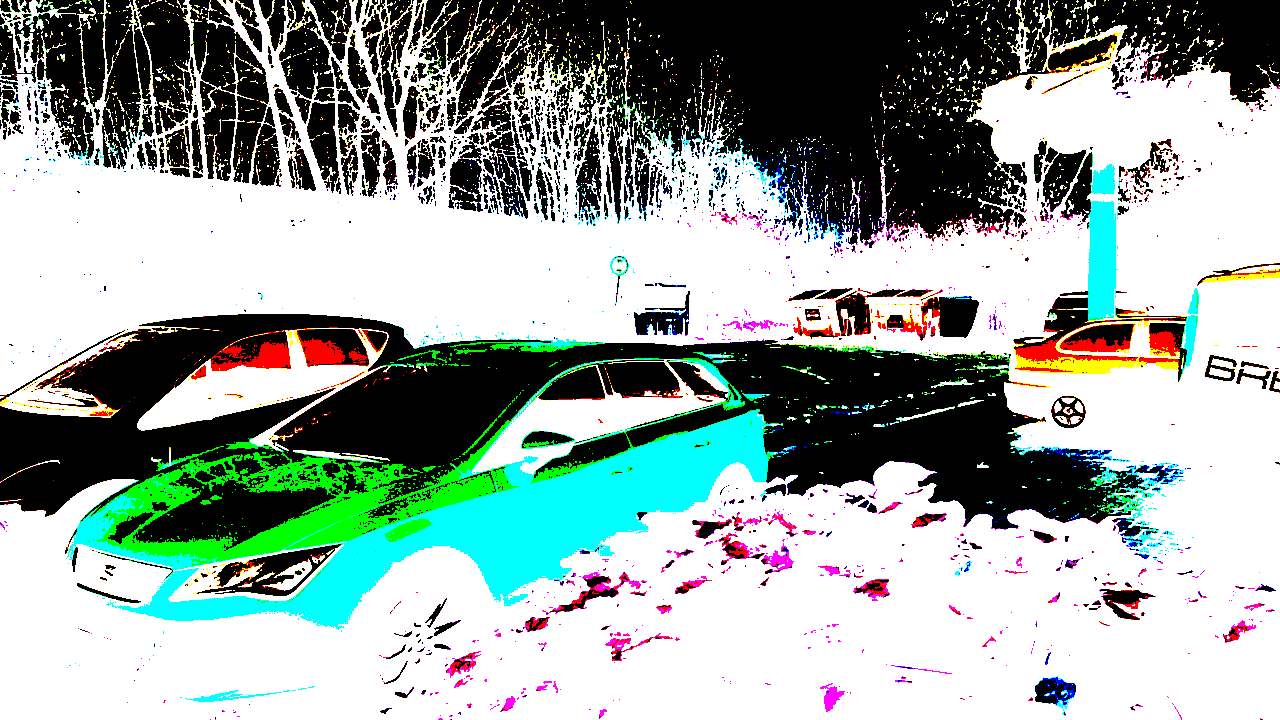
\includegraphics[width=1.4\textwidth]{img/Fotos/QuantiPic_Farbwerte.png}
	\caption[QuantiPic Farbwerte]{QuantiPic im Farbwerts-Modus}
	\label{fig:quanti_farb}
\end{figure}





\end{landscape} 

%\subsection{\textbf{Produkteinsatz}}
%
%\subsubsection{Anwendungsbereiche}
%Aktuell soll die APP nur für die Studenten der \acs{HfTL} zugänglich sein, welche ein Android-Smartphone besitzen. 
%
%\subsubsection{Zielgruppen, Qualifikationsniveau}
%
%Da bei der Nutzergruppe von Studenten mit Erfahrung im Umgang mit solchen APPs ausgegangen werden kann, wird auch die Oberfläche dementsprechend gestaltet.

\subsection{\textbf{Produktfunktionalität}}

Auszug aus der Aufgabenbeschreibung:

\textit{\glqq
Auf Basis der Analyse ist eine neue App zu programmieren,
welch die positiven Eigenschaften der vorhandenen Apps vereint und als Verarbeitungsfunktion
das Bild gleichmäßig mit einem einstellbaren Quantisierungsintervall quantisiert.\grqq
} 

\subsection{\textbf{Randbedingungen}}

Der zeitliche Rahmen für die Entwicklung und Programmierung dieser APP endet mit der 4. Kalenderwoche 2016.

%\subsection{\textbf{Annahmen und Abhängigkeiten}}
%
%Die APP wird für Android-Geräte ab Version 4.0.3 zur Verfügung gestellt.

%\subsection{\textbf{Verzögerungen}}
%
%Durch die strikte Abtrennung des zeitlichen Rahmens auf das \acs{SoSe15} darf es über diesen Zeitraum hinaus nicht zu Verzögerungen kommen

%\section{Anwendungsszenarien}
%
%\subsection{\textbf{Beschreibung aus der Nutzersicht}}
%
%Die Benutzeroberfläche muss intuitiv bedienbar sein. Der strukturierte Aufbau durch Kategorien (News, Noten, Stundenplan) soll die Übersichtlichkeit erhöhen.
%Die Logindaten werden verschlüsselt auf dem Smartphone gespeichert und auch verschlüsselt übertragen.
%Durch eine durchgehende und vollständige Dokumentation soll eine Wartung auch durch spätere Matrikel oder Administratoren der Hochschule möglich sein.
%Eine Implementierung weiterer Funktionen soll auch im Nachhinein möglich sein.

\section{Anforderungen}

\subsection{\textbf{Fachkonzept}}
Die \acs{QuantiPig}-APP  wird in Java programmiert, um durch Verwendung bestehender Klassen die Erweiterbarkeit und Realisierbarkeit zu vereinfachen. Für das Design werden \acs{XML}-Stylesheets verwendet.
\\
\\
\textbf{Verwendete Bibliotheken von Drittanbieteren}
\begin{itemize}
	\item OpenCV 
\end{itemize}

%\subsubsection{betrachtete Quantisierungsverfahren}
%
%
%Ein digitales Bild ist immer nur eine Annäherung (Approximation) der Originalabbildung.
%Bei einem technischen bildverarbeitenden System wird  (heute) fast ausschließlich ein
%kartesisches Basisgitter für das Bildraster benutzt. In der Biologie komme diese Basisgitter oft, wie zum Beispiel die Photorezeptoren im Auge, in einer Wabenstruktur vor. Bei technischen Anwendungen wird ein hexagonales Gitter verwendet.[3]
% Für die technische Bildverarbeitung werden rechteckige bzw. quadratische Strukturen verwendet, sogenannte Pixel. Somit wird eine einfache mathematische Behandlung über Matrizen ermöglicht.
% \\
% \\
%\textbf{Quantisierung}
%\\
%\\
%Unter Quantisierung versteht man die Bewertung der Helligkeit (Intensität) eines Pixels mittels einer
%festgelegten Grauwert- bzw. Farben-Menge, z.B. natürliche Zahlen von 0 bis 255.
%\\
% \\
% \textbf{Skalare Quantisierung} 
% \\
% \\
%Die skalare Quantisierung ordnet jedem Eingangswert einen quantisierten Wert aus einer endlichen Wertemenge zu. Die Zuordnung erfolgt dabei im einfachsten Fall linear auf Basis eines Rasters mit 
%Intervallen fester Länge. Durch die Abbildung aller Eingangswerte innerhalb eines bestimmten Intervalls auf denselben quantisierten Wert entsteht verlustbehaftete Datenkompression. Um bestimmte Werte stärker zu quantisieren als andere, können anstelle eines festen Rasters auch unterschiedliche Intervallbreiten gewählt werden. Durch die Einschränkungen der menschlichen Wahrnehmung kann es beispielsweise Sinn machen unterschiedliche Intervallbreiten zu verwenden. Dieses Verfahren wird als nichtlineare Quantisierung bezeichnet. [1]
%\\
%\\
%\textbf{Vektorquantisierung}
%\\
%\\
%Die Vektorquantisierung berücksichtigt mehre Signalwerte gleichzeitig, die als Vektor des mehrdimensionalen Raums aufgefasst werden. Wie die skalare Quantisierung stellt auch die Vektorquantisierung einen verlustbehafteten Vorgang dar. Ein Vektorquantisierer bildet Eingabevektoren auf eine endliche Menge ab, die aus Ausgabevektoren besteht. Für die Wahl der Ausgabevektoren können verschiedene Kriterien herangezogen werden. Im einfachsten Fall kommt das euklidische Abstandsmaß der Vektoren zum Einsatz. Die Menge der Ausgabevektoren wird als Codebuch bezeichnet. Die größte Herausforderung bei der Vektorquantisierung ist die Wahl eines geeigneten Codebuchs. Dieses muss in einer Trainingsphase mit Hilfe charakteristischer Signalvektoren optimiert und so an typische Signalstatistiken angepasst werden. Ein verbreiteter Algorithmus zur Codebuch-Erstellung ist der LBG-Algorithmus. 
%\\
%\\
%\textbf{verwendetes Verfahren}
%\\
%\\
%Auf Grund der einfacheren Implementierung haben wir uns für die skalare Quantisierung entschieden,
%
%\begin{figure}[h]
%	\centering
%		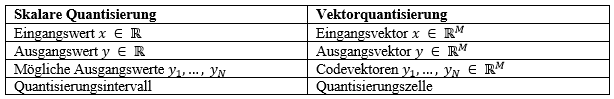
\includegraphics[width=1.0\textwidth]{img/Stephan.png}
%	\caption[Quantisierungsverfahren]{[2]Quantisierungsverfahren}
%	\label{fig:stephan_quant}
%\end{figure}
%
%[1] 'Kompendium Medieninformatik: Mediennetze,Roland Schmitz, Roland Kiefer, Johannes Maucher, Jan Schulze, Thomas Suchy, Springer-Verlag, 2006'
%
%[2] 'Signaltheorie und Kodierung,Peter Vogel,Springer-Verlag,2013'
%
%[3] '(http://www.golem.de/news/facettenaugen-forscher-entwickeln-insektenauge-fuer-drohnen-1508-115588.html'


\subsection{\textbf{Installationsprozedur}}

Die \acs{APP} wird als .apk Datei ausgeliefert und kann somit manuell auf Android-Smartphones ab Version 4.4.2 installiert werden.
Dabei muss das Installieren von Software mit unbekannter Herkunft erlaubt werden.


%\subsection{\textbf{Qualitätsanforderungen}}
%
%\subsubsection{Qualitätsmerkmale}
%Folgende Qualitätsansprüche werden gestellt:
%\begin{itemize}
%	\item Hohe Zuverlässigkeit der Software
%	\item schnelle und zuverlässige Verarbeitung der gewünschten Daten
%	\item Fehler werden mit einer entsprechenden Fehlermeldung beantwortet
%	\item Intuitiv benutzbar
%	\item Leicht zu warten und zu erweitern
%	\item Vollständige Dokumentation des Projektes
%\end{itemize}


\subsection{\textbf{Anforderung an die Entwicklung}}

\subsubsection{Entwicklungs-Umgebung}
Für die Entwicklung wird Android Studio inkl. Gradle genutzt. Für die Dokumentation und Projektkoordination wird GitHub verwendet.
Die Dokumentation wird mittels \LaTeX{} erstellt.



%\subsubsection{Projekt-Organisation}
%Die Projektorganisation wird wie in folgender Abbildung strukturiert. Als Vorgehensmodell wird das Spiralmodell mit Prototyping gewählt. Es ist ein iteratives Modell, wobei jeder Zyklus in den einzelnen Quadranten folgende Aktivitäten enthält:
%
%\begin{itemize}
%	\item Festlegung von Zielen, Identifikation von Alternativen und Beschreibung von Rahmenbedingungen
%	\item Evaluierung der Alternativen und das Erkennen, Abschätzen und Reduzieren von Risiken, z. B. durch Analysen, Simulationen oder Prototyping
%	\item Realisierung und Überprüfung des Zwischenprodukts
%	\item Planung des nächsten Zyklus der Projektfortsetzung.
%\end{itemize}
%
%Die einzelnen Aufgaben werden Personen zugeordnet. In wöchentlichen Online-Meetings über Teamviewer stellt jeder seine Ergebnisse vor und es werden diese bewertet. Anhand dieser Ergebnisse werden für den neuen Zyklus Aufgaben verteilt. Der Protokollführer hält alle Ergebnisse und Aufgaben fest und legt die Protokolle im Projektordner ab.
%
%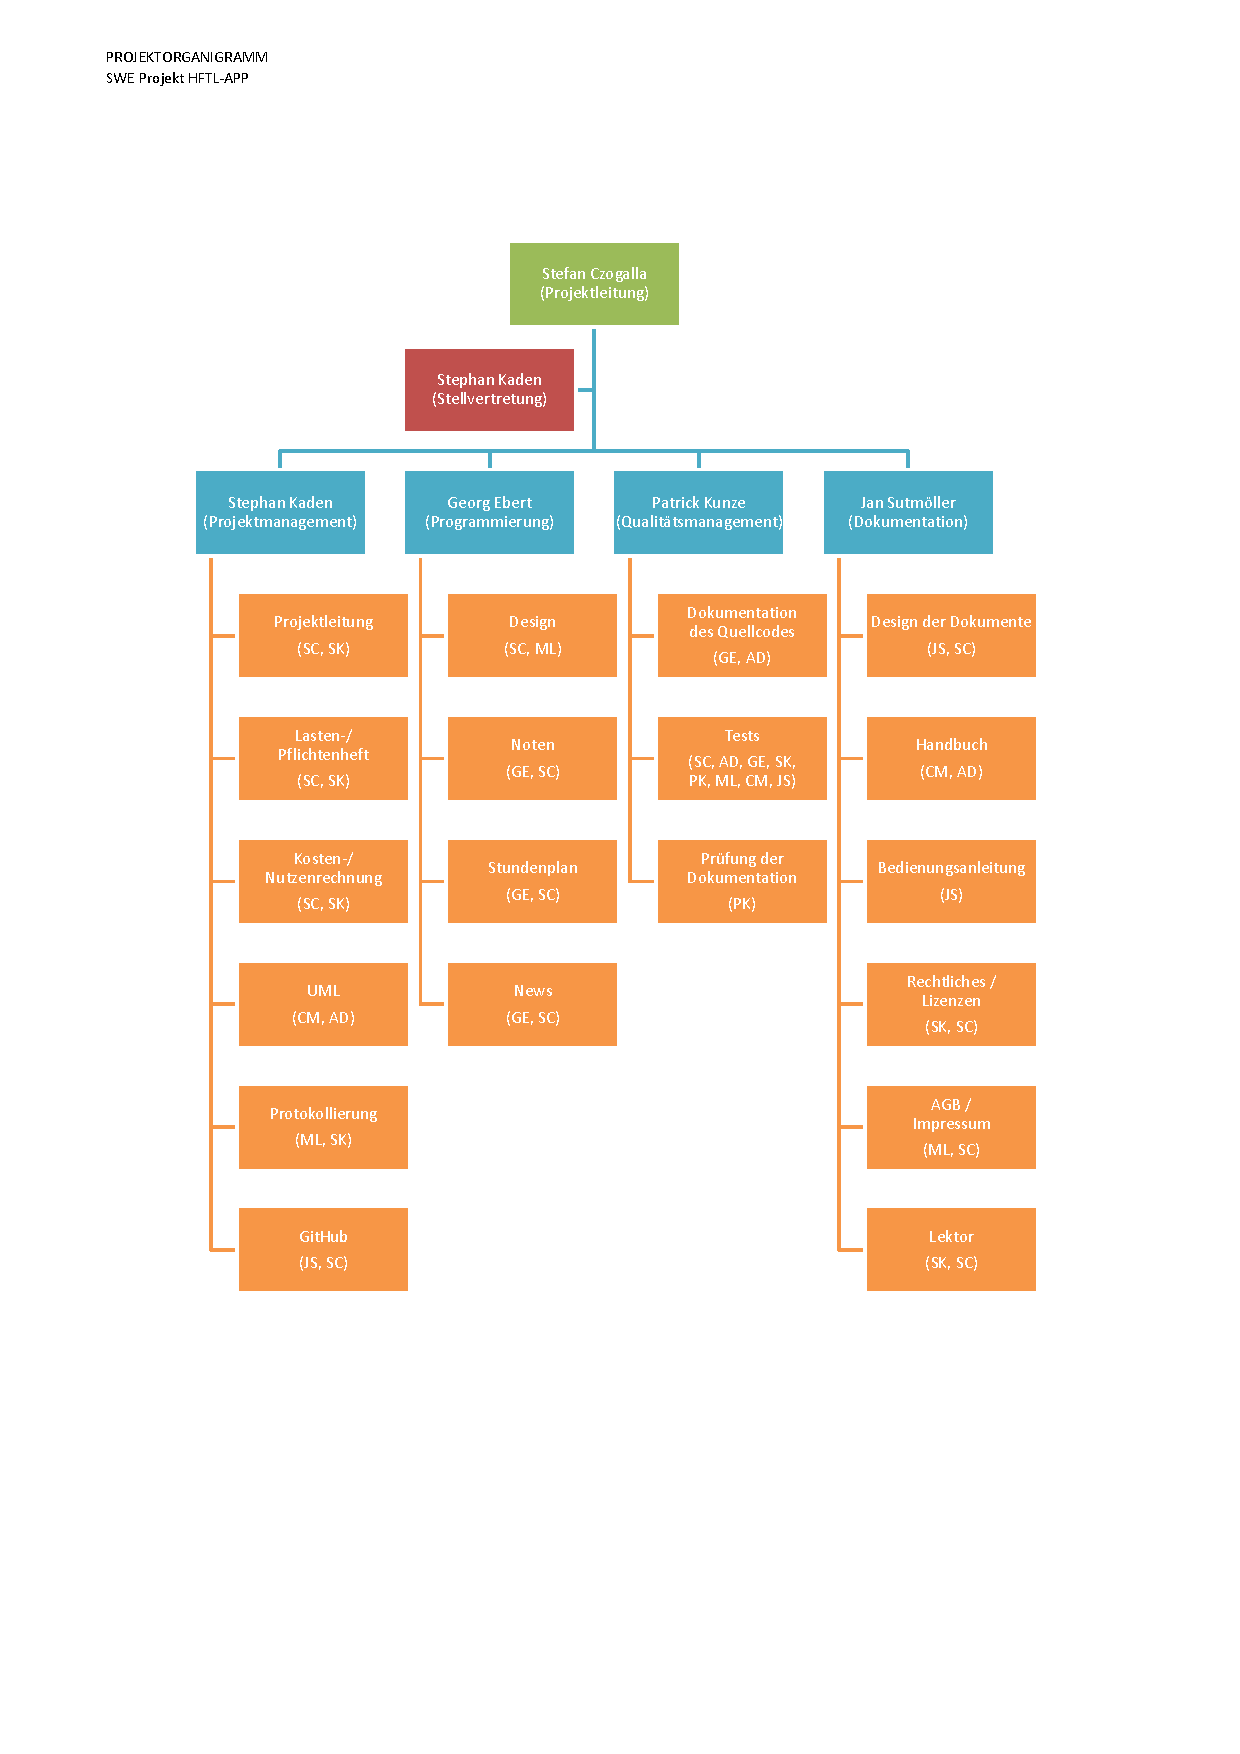
\includepdf[pages=-,noautoscale]{04_Anhang/files/swe_organigramm2.pdf}
%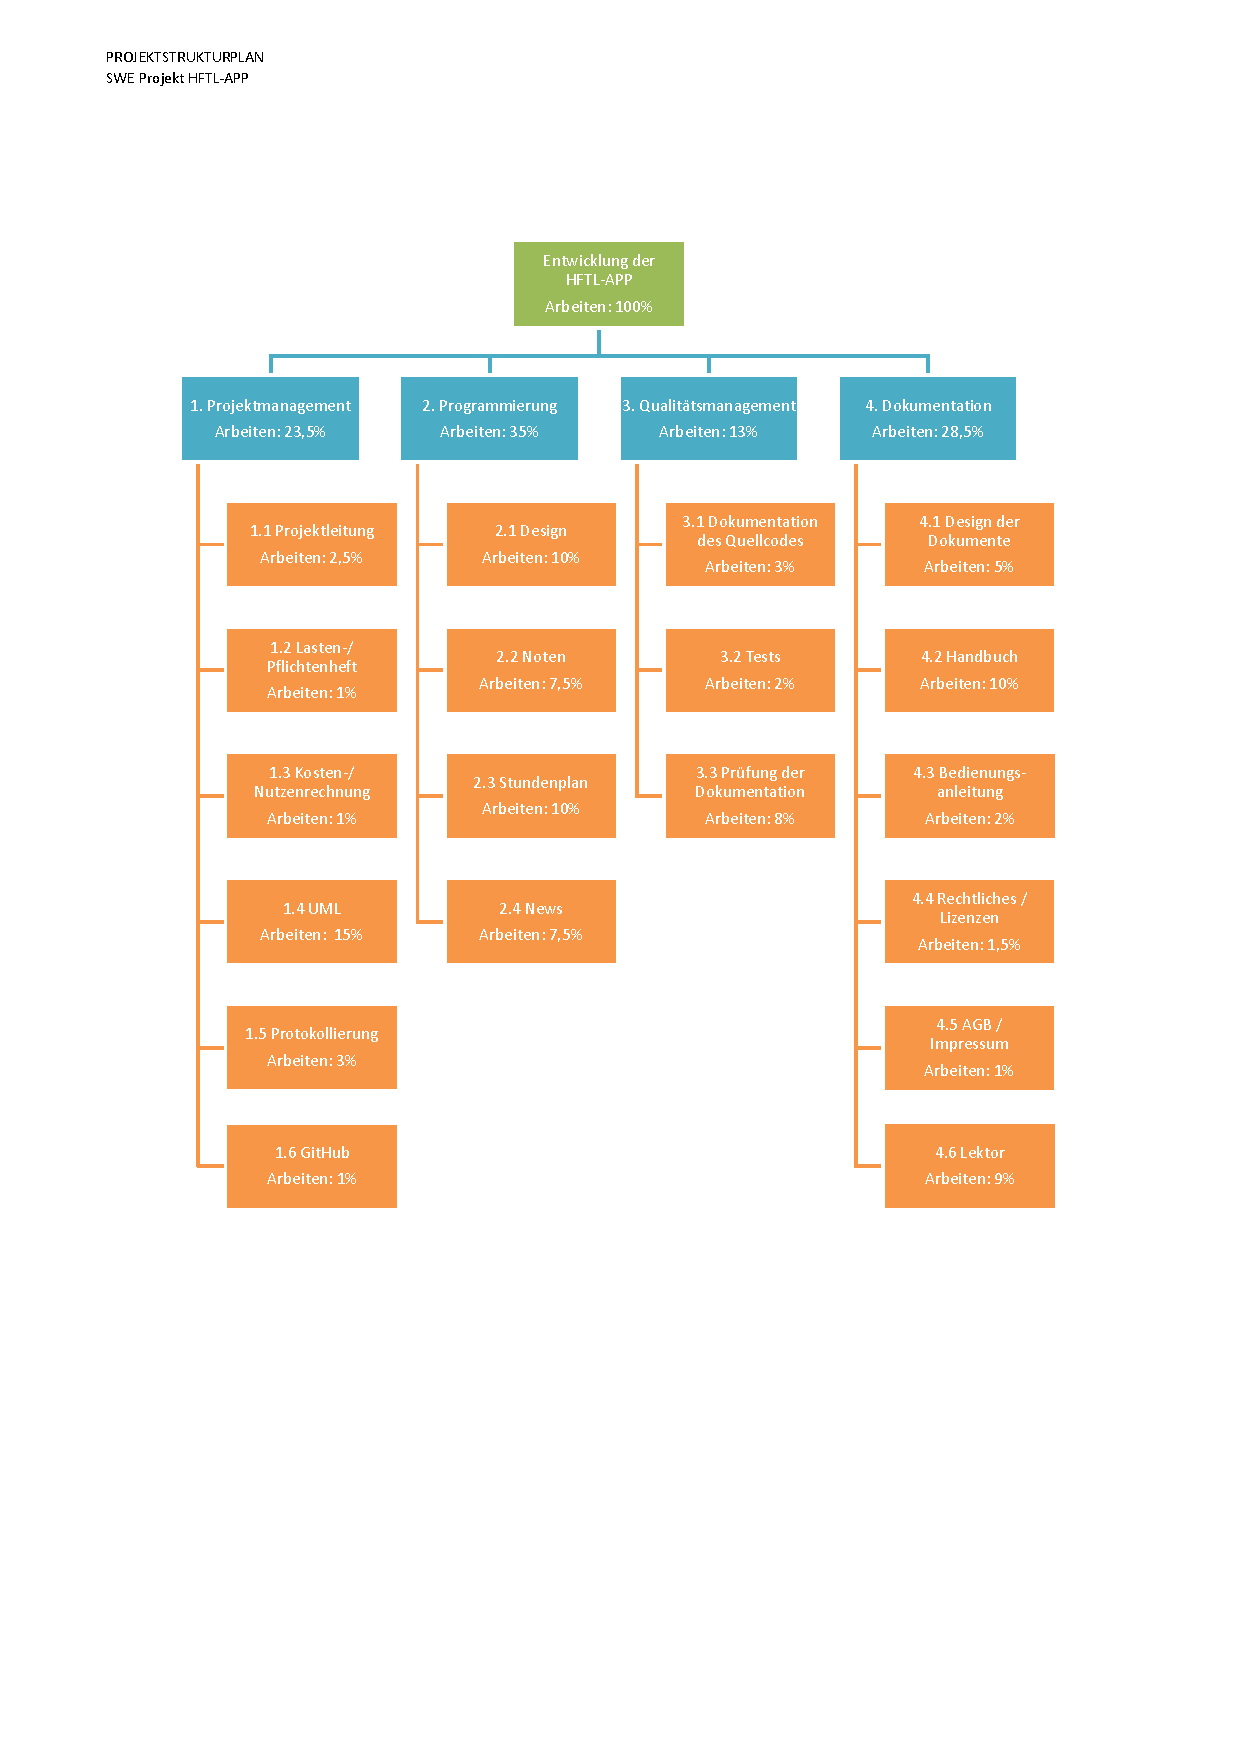
\includepdf[pages=-,noautoscale]{04_Anhang/files/swe_projektstrukturplan.pdf}


%\subsubsection{Projekt-Planung}
%siehe Anhang "'Gantt"' \ref{subsec:Gantt}

\subsubsection{Änderungsmanagement}
Zur Versionsverwaltung wurde Git eingesetzt. Als Hosting-Anbieter wurde dabei auf GitHub gesetzt, welcher einen kostenfreien Zugang für nicht kommerzielle Projekte bereitstellt. Ein \ac{GUI} oder ein Konsolenprogramm für Windows und Linux übernehmen dabei die Steuerung der Versionsverwaltung. Konflikte in den einzelnen Versionen können nur über die Konsole behoben werden. Auf der Webseite von GitHub können Milestones erstellt werden und an die jeweiligen Mitarbeiter zugeteilt werden. In den Milestones werden einzelne Aufgaben, sogenannte Issues angelegt und wiederum den Bearbeitern zugeordnet, somit ist der Bearbeitungsstand zu jeder Zeit des Projektes ersichtlich und es kann schnell auf sich ergebende Probleme reagiert werden.



%\subsubsection{Testanforderungen}
%siehe Anhang "'Testprotokollentwurf"' \ref{subsec:Testprotokollentwurf}

\section{Ergebnis}
\subsection{Übernommene Funktionalitäten}

Basierend auf den Ergebnissen des App-Vergleichs, wurden die Funktionalitäten von folgenden Apps übernommen:
\begin{description}
\item[QuanPic]~\par
\begin{itemize}
\item Um eine zusätzliche Installation des OpenCV-Managers (neben der eigentlichen App) auf das Smartphone überflüssig zu machen, wurde der grundlegende Rahmen dieser App übernommen, da diese als einzige der drei vorgegebenen Apps jene Funktionalität unterstützt.
\item Mit der Übernahme des Rahmens von "'QuanPic"' wird im Live-Bild auch die Frame-Rate und die Displayauflösung angezeigt.
\end{itemize}

\item[QuantiPic]~\par
\begin{itemize}
\item Aus dieser App wurde die grundlegende Menüführung übernommen. So werden auch in der App "'QuantiPig"' die Auswahl der Modi und des Intervalls via \textit{AlertDialog} abgefragt.
\end{itemize}

\item[FotoQuant]~\par
\begin{itemize}
\item Das Speichern der Bilder in entsprechende Ordner, je nach ausgewähltem Verfahren, sowie die Übernahme des Zeitstempels des aufgenommenen Bildes wurde aus "'FotoQuant"' übernommen.
\item Der Modus "'Midtread"' wurde grundlegend übernommen, jedoch modifiziert.
\end{itemize}


\subsection{Nicht übernommene Funktionalitäten}

Da jede der vorgegebenen Apps jeweils 2 Modi (neben der Darstellung des Originalbildes) enthielt, wurde sich nach mehreren Tests gegen folgende Verfahren entschieden:

\item[QuanPic]~\par
\begin{itemize}
\item MedianBlur 
	\begin{itemize}
	\item Ein Filterverfahren zur Kantenglättung aus der OpenCV-Bibliothek (s. \href{http://docs.opencv.org/2.4/doc/tutorials/imgproc/gausian_median_blur_bilateral_filter/gausian_median_blur_bilateral_filter.html}{OpenCV-Dokumentation})
	\end{itemize}
\item NeuQuant 
	\begin{itemize}
	\item Farbquantisierung auf Basis eines künstlichen neuronalen Netzes (s. \href{https://de.wikipedia.org/wiki/Selbstorganisierende_Karte}{Kohonennetz(Wikipedia)}) 
	\item zu leistungsschwach
	\end{itemize}
\end{itemize}

\item[QuantiPic]~\par
\begin{itemize}
\item Helligkeit
\item Farbwerte
	\begin{itemize}
	\item Farbquantisierung durch Festlegung von Schwellwerten 
	\item Vorgerfertigte Methode aus der OpenCV-Bibliothek und damit kaum modifizierbar.(s. \href{http://docs.opencv.org/2.4/doc/tutorials/imgproc/gausian_median_blur_bilateral_filter/gausian_median_blur_bilateral_filter.html}{OpenCV-Dokumentation})
	\item Die Implementierung, so wie sie in QuantiPic ist, zeigt ein Negativ mit 8 Farben. 
\end{itemize}
\end{itemize}

\item[FotoQuant]~\par
\begin{itemize}
\item Lloyd
	\begin{itemize}
	\item Vektorquantisierung auf Basis des Lloyd-Algorithmus (s. \href{https://de.wikipedia.org/wiki/K-Means-Algorithmus}{K-Means-Algorithmus(Wikipedia)})
	\item zu leistungsschwach
\end{itemize}
\end{itemize}


\subsection{Eigene Entwicklungen}

Da laut Aufgabenstellung eine Quantisierung mit \textbf{einstellbarem Intervall} gefordert war und dies in keiner der drei vorgegebenen Apps realisiert wurde, musste hier ein eigenes Verfahren implementiert werden. (\textit{s. setCluster})\\



\subsection{Umfang der APP}

\begin{figure}[h]
	\centering
		
\includegraphics[width=0.25\textwidth]{img/ic_launcher.png}
	\caption[QuantiPig Logo]{QuantiPig Logo}
	\label{fig:pig_logo}
\end{figure}

Die App wurde, angelehnt an die Namen der vorhandenen Apps, "QuantiPig" genannt. Als Logo wurde ein Schweinekopf gewählt.(siehe Abbildung \ref{fig:pig_logo})

Als Algorithmen wurden folgende Verfahren implementiert:

\begin{itemize}
	\item keine Quantisierung
	\item Pixel  
	\item Skalar
\end{itemize}

Die Modi "'Pixel"' und "'Skalar"' können jeweils mit folgenden auswählbaren Intervallen verändert werden:
\begin{itemize}
	\item 1
	\item 2
	\item 4
	\item 8
\end{itemize}


\subsection{Erscheinungsbild}
Die APP startet generell im Landscape-Modus. Wie in Abbildung \ref{fig:pig_menue} zu sehen, gibt es jeweils einen Button für die Wahl des Quantisierungsverfahrens und den Auslöser. Eine kleine Anzeige informiert über die aktuelle Bildrate und die Auflösung

\begin{figure}[h]
	\centering
		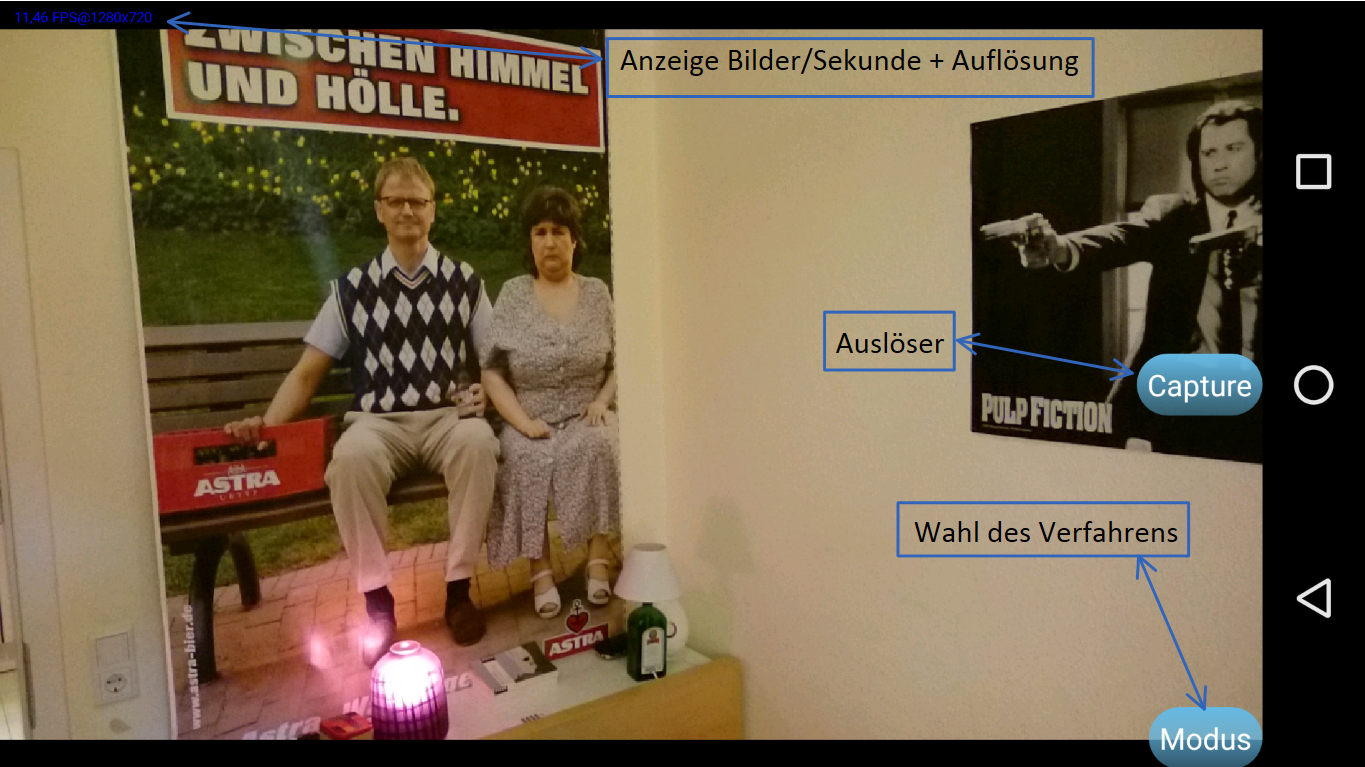
\includegraphics[width=1.0\textwidth]{img/Startbildschirm_QuantiPig.png}
	\caption[QuantiPig Startbildschirm]{QuantiPig Startbildschirm}
	\label{fig:pig_menue}
\end{figure}

Nach Drücken auf den Auslöser wird ein Foto mit aktuellem Verfahren gemacht und in den entsprechenden Ordner auf dem Smartphone abgelegt. Als Name wird das jeweilige Verfahren, gefolgt von einem Zeitstempel verwendet.

Nach betätigen des Buttons \glqq
Modus\grqq
, öffnet sich, wie in Abbildung \ref{fig:pig_verfahren} zu sehen, ein Auswahlmenü für die drei verschiedenen Verfahren.

\begin{figure}[h!]
	\centering
		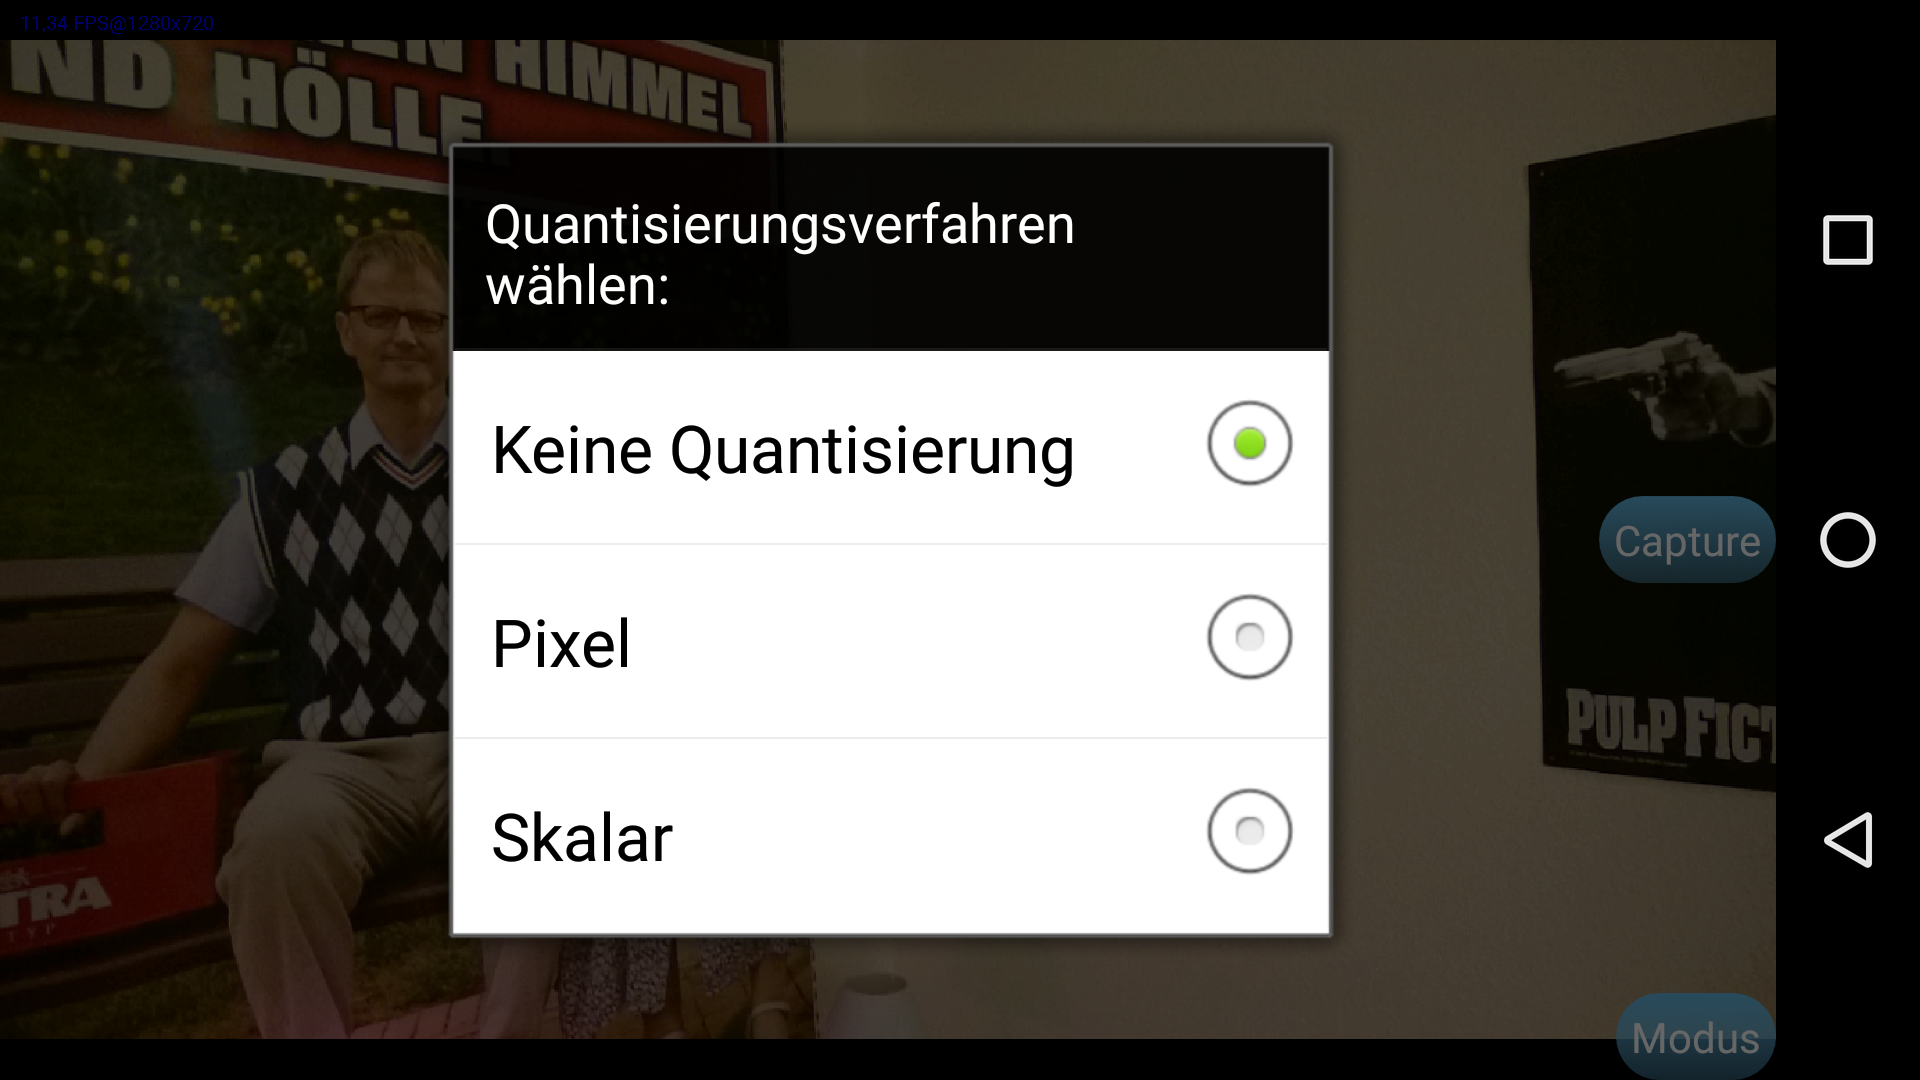
\includegraphics[width=1.0\textwidth]{img/Verfahren_QuantiPig.png}
	\caption[QuantiPig-Menü Verarbeitungsverfahren]{QuantiPig-Menü Verarbeitungsverfahren}
	\label{fig:pig_verfahren}
\end{figure}

Im Modus "'Pixel"' und "'Skalar"' (siehe Abbildung \ref{fig:pig_intervall}) gibt es einen weiteren Button mit dem man das Intervall auswählen kann.

\begin{figure}[h!]
	\centering
		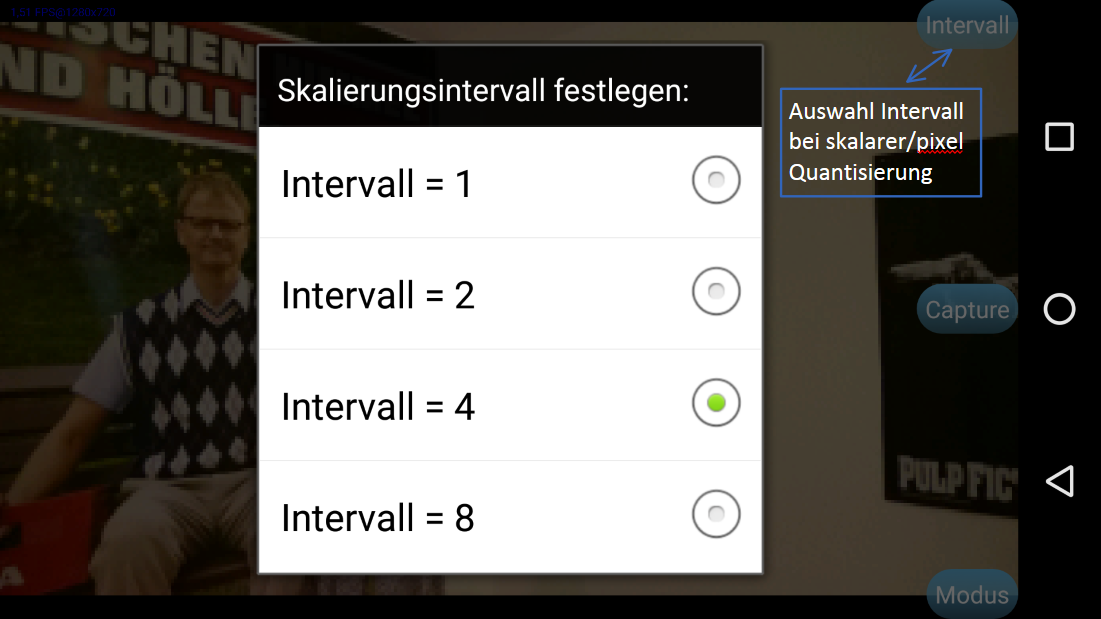
\includegraphics[width=1.0\textwidth]{img/Intervall_QuantiPig.png}
	\caption[QuantiPig-Menü Quantisierungsintervall]{QuantiPig-Menü Quantisierungsintervall}
	\label{fig:pig_intervall}
\end{figure}


\clearpage

\newpage
\subsection{Quellcode}
\subsubsection{Allgemein}

Wie bereits erwähnt wurde der grundlegende Aufbau aus der App "'QuanPic"' übernommen. Neben der Hauptklasse wurde für die beiden Bearbeitungsmodi jeweils eine eigene Klasse erstellt:
\begin{itemize}
	\item MainActivity.java
	\item Pixel.java
	\item Skalar.java
\end{itemize}
Im Folgenden wird nicht auf jedes Detail im Quellcode eingegangen, jedoch die wichtigsten Funktionen erläutert.

\subsubsection{MainActivity.java}
\label{mainactivity}

Die MainActivity ist die Haupt- und damit Startaktivität der App. Hauptaufgabe der Aktivität ist es, Objekte  (Strings, Buttons, Menüs, Ladebalken etc.) beim Start der App aufzurufen und ggf. mit Aktions-Listener zu versehen, sofern die Objekte hier auf Nutzereingaben reagieren sollen. \\
Dies geschieht innerhalb der Methode "'\textit{onCreate();}"', die das Layout einer View zuordnet und anschließend bereits erwähnte Objekte instanziert. \\
\\
Folgender Ausschnitt zeigt am Beispiel von mCameraView, wie dieses einem Layoutobjekt (\textcolor{lila}{\textit{suface\_view}})  zugeordnet wird, die Sichtbarkeit manipuliert wird und mit dem \hyperref[CameraListener]{CameraListener}  bestückt wird:

\lstset{language = JAVA}

\begin{lstlisting}
setContentView(quantipig.R.layout.activity_main);
mCameraView = (CameraBridgeViewBase) findViewById(R.id.surface_view);
\end{lstlisting}

Darüber hinaus sind hier einige wichtige Methoden aufgeführt, die essentiell für die Funktionsweise von OpenCV und somit für die App als funktionierende Smartphone-Kamera sind:
\begin{itemize}
\item onResume()
\item BaseLoaderCallback()
\item onPause()
\item onDestroy()
\item onStart()
\end{itemize}
Weitere Details können auch der \href{http://docs.opencv.org/2.4/doc/tutorials/introduction/android_binary_package/dev_with_OCV_on_Android.html#dev-with-ocv-on-android}{OpenCV-Dokumentation} entnommen werden.

\item[imageProcessing()]~\par
\label{imageProcessing}

Diese Methode ist das Kernstück für die Bildbearbeitung der App. 
Hier sind auch die Standard-Methoden von OpenCV implementiert:
s. hierzu OpenCV-Dokumentation:
\begin{itemize}
\item \href{http://docs.opencv.org/java/2.4.9/org/opencv/android/CameraBridgeViewBase.CvCameraViewListener2.html}{CvCameraViewListener2}
\item \href{http://docs.opencv.org/java/2.4.9/org/opencv/android/CameraBridgeViewBase.CvCameraViewFrame.html}{CvCameraViewFrame}
\end{itemize}
 Die Methode "'\textit{onCameraFrame()}"' erhält Einzelbilder von der Kamera und übergibt dieses an ein Objekt der Open-CV Klasse "'\textit{Mat}"' als RGBA-Matrix. Diese Matrix kann anschließend bearbeitet werden und wird anschließend weiter an das Display des Endgeräts gegeben. Der grundlegende Aufbau wurde aus der Vorlage "'QuantPic"' übernommen. Es wurden jedoch diverse Änderungen am Quelltext vorgenommen.\\ 
Die wichtigsten Änderungen:
\begin{itemize}
\item Speichern der Höhe, der Breite und der Anzahl der Kanäle des Live-Bildes, damit diese Werte an den jeweiligen Modus übergeben werden können.
\begin{lstlisting}
Mat mMat;
int mHeight  = inputFrame.rgba().height();
int mWidth   = inputFrame.rgba().width();
int channels = inputFrame.rgba().channels();
\end{lstlisting}

\item Änderung der Abfrage des ausgewählten Modus von einer if- zu einer \textbf{switch case} Anweisung. Dabei wird der Wert der Variable \textcolor{lila}{modeSelector} übergeben, welche wiederum den ausgewählten Modus repräsentiert und somit die Ausgabe auf dem Display entsprechend ändert.
\begin{lstlisting}
switch (modeSelector){
 case 0: (...) /* keine Quantisierung */
 case 1: (...) /* Pixel */
 case 2: (...) /* Skalar */
}
\end{lstlisting}
\item Abfrage des ausgewählten Intervalls (nur bei "'Pixel"' und "Skalar"')
\begin{lstlisting}
cluster = setCluster();
\end{lstlisting}
\item Übergabe des Live-Bildes und den ermittelten Variablen an die jeweilige Klasse zur Bearbeitung (nur bei "'Pixel"' und "Skalar"')
\begin{lstlisting}
mMat = Pixel.pixel(inputFrame.rgba(), mHeight, mWidth, channels, cluster);
\end{lstlisting}
\item Übergabe des bearbeiteten Bildes zum Speichern
\begin{lstlisting}
getsavingImage(mMat);
\end{lstlisting}
\item Übergabe des bearbeiteten Bildes an das Display
\begin{lstlisting}
return mMat;
\end{lstlisting}
\end{itemize}

\newpage

\item[getsavingImage()]~\par
\label{getsavingImage}
Diese Methode speichert das aus der Methode \hyperref[imageProcessing]{imageProcessing()} übergebene Bild und stellt es der Methode \hyperref[saveImage]{saveImage} zur Verfügung, sofern der Button zum Speichern betätigt wurde.
\begin{lstlisting}
public void getsavingImage(Mat mat) {
 previewImage = mat;
}
\end{lstlisting}

\item[setModus()]~\par
\label{setModus}
Diese Methode baut die Abfrage des Modus via AlertDialog und OnClickListener auf und übergibt entsprechend der Auswahl einen Wert an die Variable \textcolor{lila}{modeSelector}, welche wiederum von der Methode \hyperref[imageProcessing]{imageProcessing()} ausgelesen wird.\\
Die Abfrage erfolgt wiederum über eine switch case Anweisung. Ausschlaggebend ist der Wert der Variable \textcolor{lila}{quantizationMode}.\\
Je nach ausgewähltem Modus wird noch der Intervall-Button aus- (\textit{KeineQuantisierung}) oder eingeblendet (\textit{Pixel, Skalar}.
\begin{lstlisting}
switch (quantizationMode) {
 case QUANT_MODE_0: { /* Keine Quantisierung	*/
  hideButton();       /* Verstecke Intervall-Button */
  modeSelector = 0;
  break;
 }
 case QUANT_MODE_1: { /* Pixel */
  showButton();       /* Zeige Intervall-Button */
  modeSelector = 1;
  break;
 }
 (...)
}
\end{lstlisting}

\item[setCluster()]~\par
\label{setCluster}
Diese Methode übergibt anhand des ausgewählten Eintrags in der Methode \hyperref[createClusterMenu]{createClusterMenu()} den entsprechenden Intervall-Wert in die Variable \textcolor{lila}{cluster}.\\
Diese Intervalle werden dann von den Klassen "'Pixel"' und "'Skalar"' verwendet um unterschiedliche Ergebnisse zu erzielen.\\
Folgende Intervall-Werte gibt es:
\begin{itemize}
\item 1
\item 2
\item 4
\item 8
\end{itemize}
Als Abfragewert dient die Variable \textcolor{lila}{selectedCluster} aus der Methode \hyperref[createClusterMenu]{createClusterMenu()}.
\begin{lstlisting}
switch (selectedCluster) {
 case Cluster_0: {
  cluster = 1;
  return cluster;
 }
 (...)
} 
\end{lstlisting}

\item[createClusterMenu()]~\par
\label{createClusterMenu}
Hier wird die Abfrage des Intervalls mittels AlertDialog realisiert. Der Ausgewählte Wert wird schließlich von der Methode \hyperref[setCluster]{setCluster} verwendet.

\item[saveImage()]~\par
\label{saveImage}
Sobald der Button "'Capture"' betätigt wurde, wird das (bearbeitete) Bild in diese Methode übergeben und zum Speichern als .png-Datei vorbereitet.\\
Dabei wird zunächst der aktuelle Zeitpunkt ermittelt und gespeichert. 
\begin{lstlisting}
SimpleDateFormat sdf = new SimpleDateFormat("yy_MM_dd-HH_mm_ss");
String currentDateAndTime = sdf.format(new Date());
\end{lstlisting}


Anschließend wird das Bild von RGBA in einen BGRA-Farbraum konvertiert, da sonst das gespeicherte Bild vom angezeigten Bild auf dem Display abweicht (Blau wird als Rot dargestellt und umgekehrt). 
\begin{lstlisting}
Imgproc.cvtColor(mat, mat, Imgproc.COLOR_RGBA2BGRA, 4);
\end{lstlisting}
Entsprechend des ausgewählten Modus und Intervalls wird nun der Pfad- und Dateiname erstellt.\\
Alle Bilder werden unter DCIM/QuantiPig/ gespeichert.\\
Am Beispiel für Modus 1 (Pixel):
\begin{lstlisting}
rootPath = new File(Environment.getExternalStoragePublicDirectory(Environment.DIRECTORY_DCIM).getPath() + "/QuantiPig/Pixel");
fileName = QUANT_MODE_1_STRING + "-" + cluster + "_" + currentDateAndTime + ".png";
\end{lstlisting}
Als Resultat wird das Bild in den Ordner \textit{DCIM/QuantiPig/Pixel} gespeichert.
Der Dateiname lautet dann beispielsweise: \textit{Pixel-8\_15\_12\_24-18\_59\_30.png}

\newpage

\subsubsection{Pixel.java}
\label{Pixel}
Diese Klasse dient als Container für die Methode \textit{pixel()}.\\
Die Methode geht dabei wie folgt vor:
\begin{itemize}
\item Es werden Quadrate der Kantenlänge = Intervall auf das Originalbild gelegt.
\item Der durchschnittliche Farbwert aller Bildpunkte innerhalb des Quadrats wird gebildet
\item Die Bildpunkte des Quadrates werden nun mit dem Durchschnittsfarbwert überschrieben.
\end{itemize}
Bei (Intervall > 1) entsteht der Eindruck, dass die Auflösung des Displays gesenkt wird und somit das Bild "'verpixelt"' wird. Bei steigendem Intervall wird der Effekt deutlicher. \\

\item[pixel]~\par
\label{pixel}
Der äußere Rahmen der Methode. Es wird das Bild der Kamera, seine Maße, die Anzahl der Kanäle und das ausgewählte Intervall übergeben.
\\\
\begin{lstlisting}
public static Mat pixel(Mat mat, int mHeight, int mWidth, int channels, int intervall){ 
	...
	return mat;
} 
\end{lstlisting}

Zur einfacheren Handhabe wird das übergebene Bild in ein Byte-Array geschrieben.
\begin{lstlisting}
 byte[] buff = new byte[mHeight * mWidth * channels];
 mat.get(0, 0, buff);
\end{lstlisting}

Zunächst werden einige Variablen mit \textcolor{blau}{0} instanziert.
\begin{lstlisting}
 int x = 0;
 int k = 0;                                                                                  
 int countY = 0;                                                                             
 int[] frame = new int[mWidth / cluster * mHeight / cluster * channels];                            
\end{lstlisting}
Kurze Eräuterung:
\begin{itemize}
\item x: Index des abzutastenden Farbwertes auf buff
\item k: Index des RGBA-Bildpunktes des Hilfsarrays frame
\item countY: Zähler, wie viele Zeilen von buff schon abgetastet wurden
\item frame: Das Hifsarray zur Berechnung des Durchschnitts.   
\end{itemize}
Nun beginnt das Abtasten und das Überschreiben der Werte aus buff in frame mit Hilfe von vier ineinander verschachtelten Schleifen.\\
Die äußere Schleife geht vertikal, also zeilenweise das Bild runter:
\begin{lstlisting}
 for (int n = 0; n < mHeight; n++) {                                                         
\end{lstlisting}
Es ist notwendig die Anzahl abgetasteten Zeilen zu kennen. Daher wird jeder Schleifendurchlauf der äußeren Schleife mitgezählt.
\begin{lstlisting}
  countY++;                                                                               
\end{lstlisting}
Nun beginnt der Schleifendurchlauf in der Horizontalen. Als erstes wird jedes Cluster einzeln durchlaufen.
\begin{lstlisting}
  for (int m = 0; m < mWidth / intervall; m++) {                                            
\end{lstlisting}
Danach wird jeder Bildpunkt im Cluster durchlaufen.
\begin{lstlisting}            
   for (int j = 0; j < intervall; j++) {                                                 
\end{lstlisting}
Und nun werden die RGBA-Kanäle des Bildpunktes durchlaufen. 
\begin{lstlisting}
    for (int i = 0; i < channels; i++) {                                                   
\end{lstlisting}
Zusammenfassung:
\begin{itemize}
\item x = Index des Quell-Arrays
\item k = Index des Ziel-Arrays
\item n = Zeile des Quell-Arrays
\item m = Index des Clusters in der Zeile
\item j = Index des Bildpunktes innerhalb des Clusters
\item i = Index des RGBA-Kanals im Bildpunkt   
\end{itemize}
Damit können nun alle Koordinaten durchlaufen werden. Die Sache wird nur noch dadurch komplizierter, da JAVA mit signed-Werten arbeitet und sich somit der Wert inhaltlich ändert. (Wertebereich ändert sich von (0 bis 255) auf (-128 bis 127))\\
Daraus folgend werden Additionen mit Werten > 127 als Subtraktion ausgeführt. Dies wird vor allem dann an Kanten sichtbar, wo stark unterschiedliche Werte dicht beieinander liegen. Dieser Effekt wird ggf durch ein großes Intervall verstärkt. (s. linkes Bild von \ref{fig:signedunsigned})\\\

Um das Problem zu umgehen und das Resultat wie im rechten Teil des Bildes zu erzielen, werden die negativen Werte umgerechnet.
\begin{lstlisting}                    
     if (buff[x + i + j * channels] >= 0)                                               
      frame[k + i] += ((int) buff[x + i + j * channels]);                            
     else
      frame[k + i] += ((int) buff[x + i + j * channels] & 0xff);                     
    }
   }
\end{lstlisting}
Mit dem Schließen der inneren beiden Schleifen wurde das erste Cluster (m=0) in der ersten Zeile vollständig abgetastet der erste Bildpunkt des Hilfsarray (zunächst) fertig befüllt. Daher wird wird der Index des Zielarrays um einen Bildpunkt, also um 4 (aufgrund der vier Kanäle) erhöht. Gleichzeitig springt der Index des Quell-Arrays auf den ersten Bildpunkt der in das neue Cluster geschrieben werden soll. Dies wird so lange gemacht, bis das Zeilenende erreicht wurde.
\begin{lstlisting}                 
                k += channels;                                                                             
                x += channels * intervall;                                                                   
            }
\end{lstlisting}
Dies wird nun Zeile für Zeile so oft wiederholt. Da der Algorithmus auch Bildpunkte eines Cluster abtasten muss, die untereinander liegen, muss nach jedem Zeilendurchlauf geprüft werden, ob die Clusterbreite (/-höhe) bereits erreicht wurde. Ist dies nicht geschehen, werden alle untereinander stehenden Werte in den selben Index des Ziel-Arrays geschrieben, womit dieser immer wieder am Zeilenanfang zurückgesetzt werden muss.
\begin{lstlisting}            
   if (countY < intervall)                                                                   
    k -= mWidth * channels / intervall;                                                          
\end{lstlisting}
Wurden nun auch in der Vertikalen alle Bildpunkte abgetastet, dürfen sich alle Indexe erhöhen. Nur das Zählen der Schleifendurchläufe, bis wieder die Clusterhöhe erreicht wurde, muss von vorne beginnen.
\begin{lstlisting}
   else
    countY = 0;                                                                         
  }
\end{lstlisting}
Nach dem nun alle Werte in das cluster-weise übertragen und im Hilfsarray aufsummiert wurden, muss nur noch der Durchschnitt berechnet werden (Summe der Elemente : Anzahl der Elemente). Bei der Methode muss man sich jedoch im Klaren sein, dass hier aufgrund des verwendeten Datentyps \textcolor{darkblue}{integer} eine Ganzzahldivision stattfindet, was am Ende zu Rundungsfehlern führt.
\begin{lstlisting}
  for (int i = 0; i < frame.length; i++) {
   frame[i] = frame[i] / (intervall * intervall);
  }
\end{lstlisting}
Nun werden die Durchschnittswerte wieder zurück in das Quell-Array geschrieben. Dabei werden die gleichen vier Schleifen wie zuvor durchlaufen. 
\begin{lstlisting}
  k = 0;
  countY = 0;
  x = 0;

  for (int n = 0; n < mHeight; n++) {
   countY++;

   for (int m = 0; m < mWidth / intervall; m++) {
    for (int j = 0; j < intervall; j++) {
     for (int i = 0; i < channels; i++) {
      buff[x + i + j * channels] = (byte) frame[k + i];
     }
    }
    k += 4;
    x += 4 * intervall;
   }
   if (countY < intervall)
    k -= mWidth * channels / intervall;
   else
    countY = 0;
  }
\end{lstlisting}
Zum Schluss wird das Byte-Array wieder zurück in das Bild geschrieben.
\begin{lstlisting}
mat.put(0, 0, buff);
\end{lstlisting}


\begin{figure}[h]
	\centering
		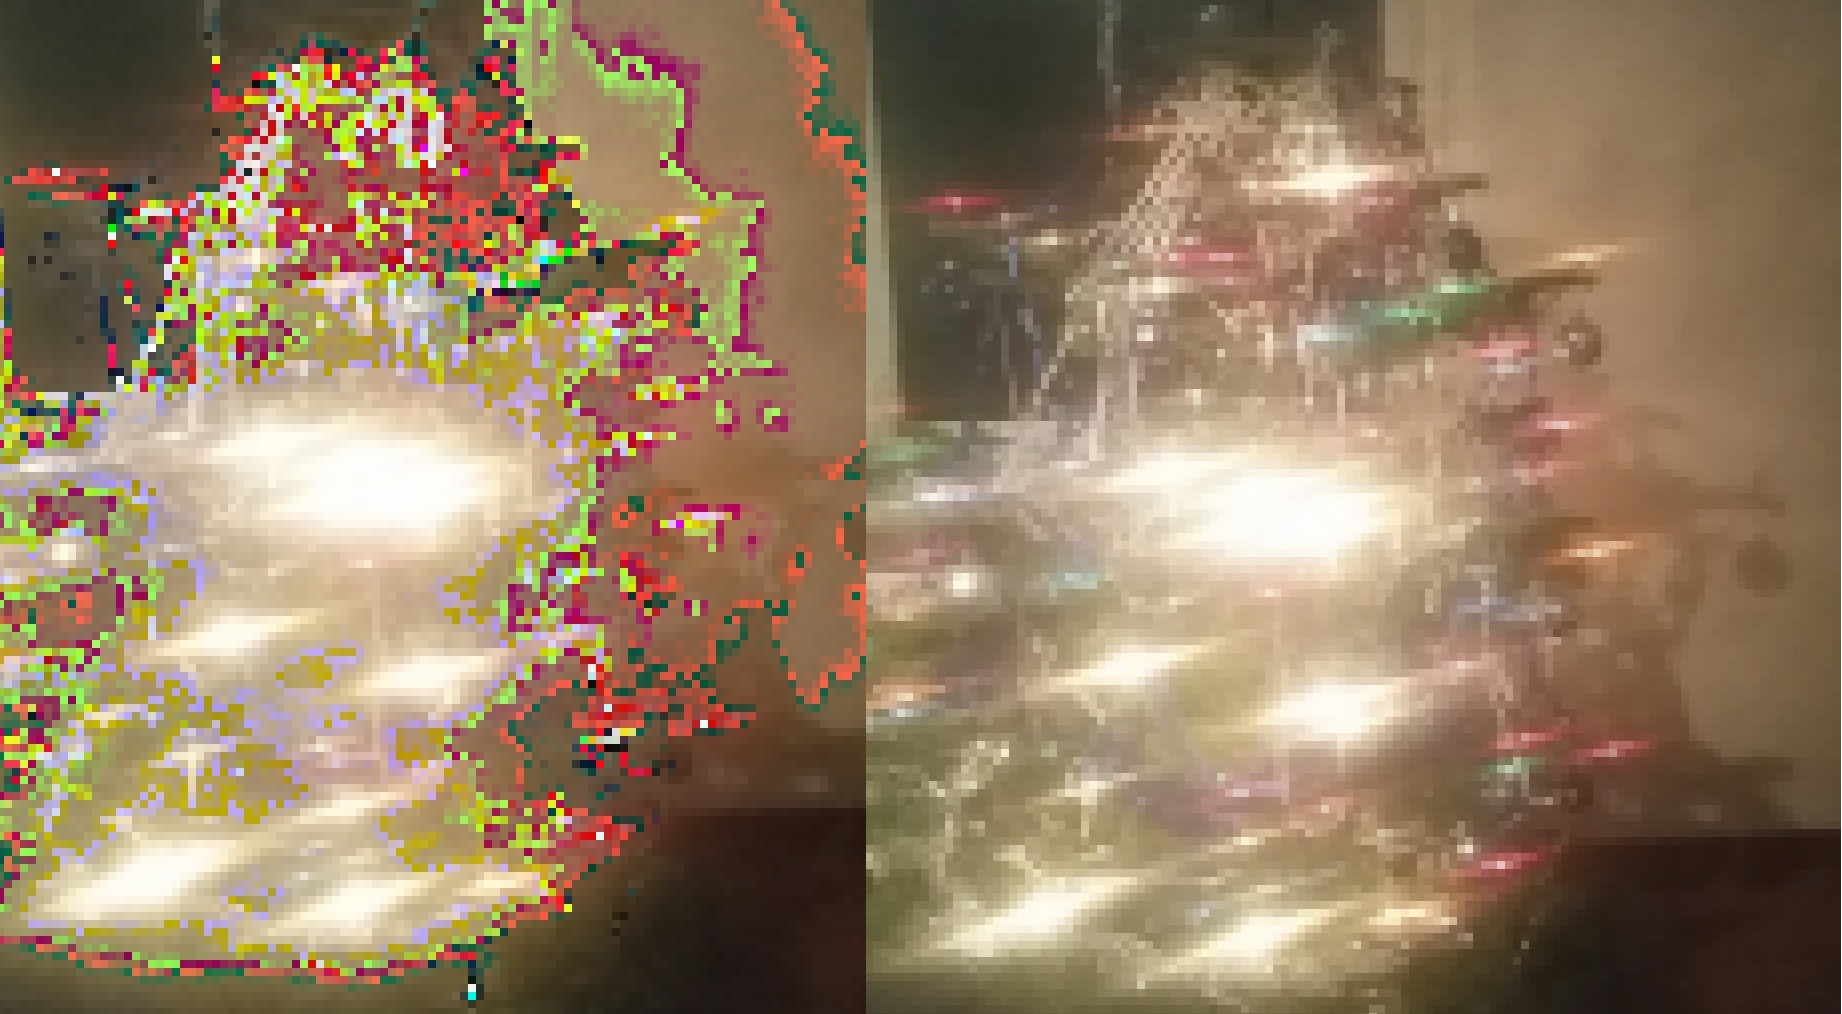
\includegraphics[width=1.0\textwidth]{img/signedUnsigned.jpg}
	\caption[signedunsigned]{Gleiches Motiv mit einem 8 x 8 Intervall aufgenommen}
	\label{fig:signedunsigned}
\end{figure}

\newpage


\subsubsection{Skalar.java}
\label{Skalar}
Diese Klasse dient als Container für die Methode "'skalar"'. Hier werden die binären Farbwerte mittels logischer Konjunktion (AND) mit einem binären Vektor \textit{v} verknüpft. Der Anzahl der daraufhin dargestellten Farben \textit{n} hängt vom gewählten Intervall \textit{i} ab.\\\ 
\( n = 2^{i^k}, mit k = Anzahl der Kanäle\) \\\
Daraus folgt, bei \(k = 3\)(RGB):
\begin{itemize}
\item Intervall = 1:  
\begin{itemize}
\item v = 1000 0000
\item \( n = 2^{1^3} =        8 \)
\end{itemize}
\item Intervall = 2:
\begin{itemize}
\item v = 1100 0000
\item \( n = 2^{2^3} =       64 \)
\end{itemize}
\item Intervall = 4:
\begin{itemize}
\item v = 1111 0000
\item \( n = 2^{4^3} =     4096 \)
\end{itemize}  
\item Intervall = 8:
\begin{itemize}
\item v = 1111 1111
\item \( n = 2^{8^3} = 16777216 \) 
\end{itemize}  
\end{itemize}
\item[skalar]~\par
\label{skalar}
Der Rahmen dieser Methode ist analog zu \hyperref[pixel]{pixel()} aufgebaut. Es werden das Originalbild (als RGBA-Matrix), die Maße, die Anzahl der Kanäle, sowie das eingestellte Intervall übergeben, in ein Byte-Array geschrieben und am Ende das modifizierte Byte-Array in das Bild geschrieben, welches dann wieder zurückgegeben wird.
\begin{lstlisting}
public static Mat skalar(Mat mat, int mHeight, int mWidth, int channels, int intervall) {
 byte[] buff = new byte[mHeight * mWidth * channels]; 
 mat.get(0, 0, buff);                                 
 
 (...) 
 
 mat.put(0, 0, buff);                                			
 return mat;                                          			
}
\end{lstlisting}

Der innere Aufbau dieser Methode ähnelt dem Modus "'Midtread"' der App "'FotoQuant"'. Es wurden jedoch einige Änderungen vorgenommen.\\
Zunächst wird ein Bitshiftvektor initialisiert. Da Java Bitshift-Operationen nur mit dem Datentyp \textcolor{blau}{Integer} (32 Bit) durchführen kann, das Byte-Array jedoch 8 Bit pro Index enthält, werden zunächst alle Bit \(B_i\) mit einem Index \(i>7\) mit \textcolor{blau}{1} initialisiert.
\begin{lstlisting}
int bitshift = 0xFFFFFF00;
\end{lstlisting} 
Danach werden die Bits in Abhängigkeit vom Intervall nach rechts verschoben (shift-right Operator)
\begin{lstlisting}
bitshift = bitshift >> intervall;
\end{lstlisting} 
Nun kommt der Aufbau, der aus "'FotoQuant"' übernommen wurde. Das Array wird abgetastet und jeder einzelne Farbwert wird modifiziert. Allerdings ist diese Modifizierung selbst wiederum anders, als in der Vorlage.
\begin{lstlisting}
int t;
for (int i = 0; i < mWidth * mHeight; i++) {
 t = i * channels;                              /* Bildpunkte */
 buff[t    ] = (byte) (buff[t    ] & bitshift); /* Rot */
 buff[t + 1] = (byte) (buff[t + 1] & bitshift); /* Gelb */
 buff[t + 2] = (byte) (buff[t + 2] & bitshift); /* Blau */
}
\end{lstlisting} 


\end{description}


\newpage



\subsection{Beispielbilder}
\begin{landscape}


\begin{figure}[h]
	\centering
		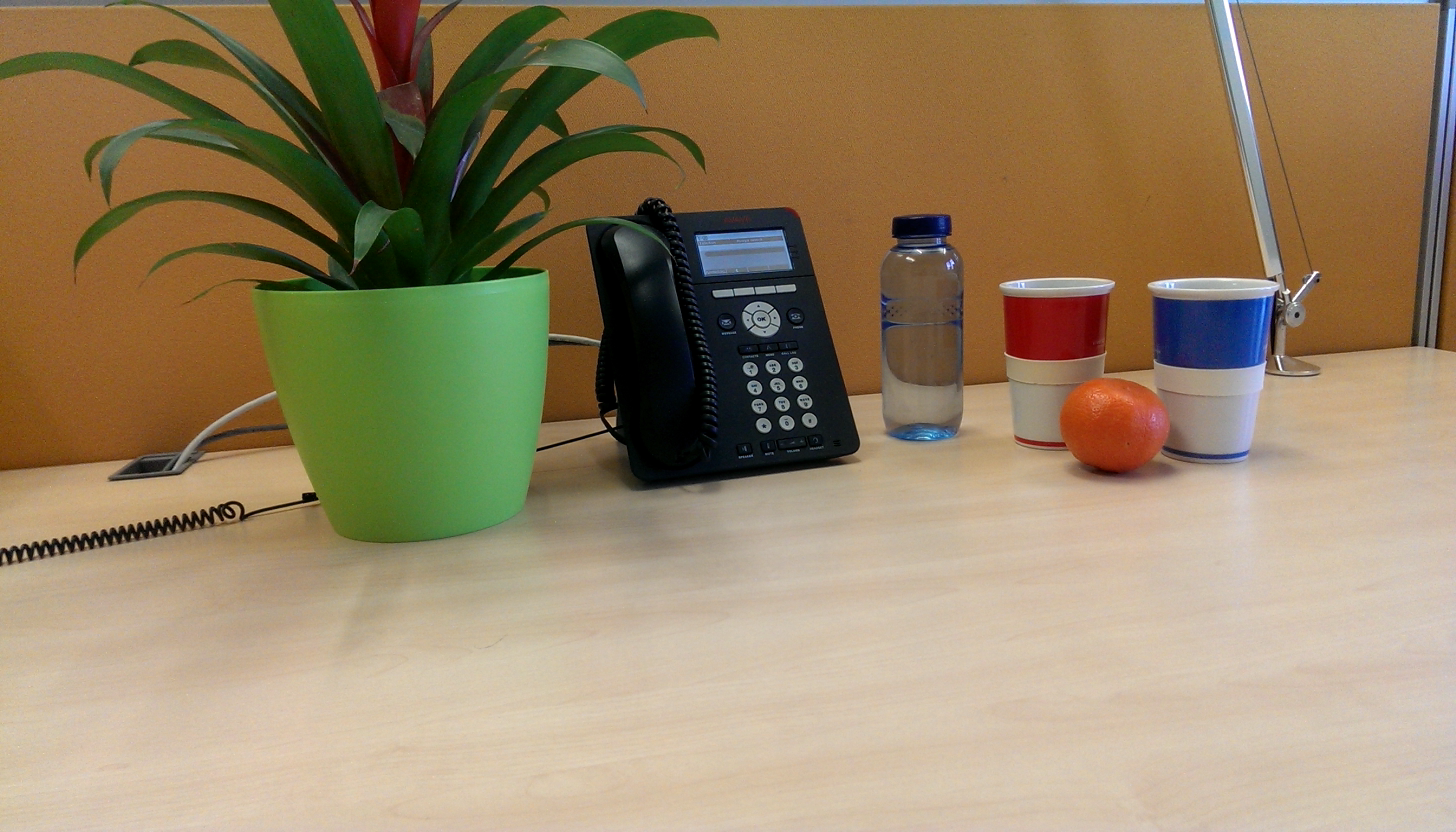
\includegraphics[width=1.4\textwidth]{img/Fotos/QuantiPig_Original.png}
	\caption[QuantiPig Originalbild]{QuantiPig Originalbild}
	\label{fig:pig_original}
\end{figure}

\begin{figure}[h]
	\centering
		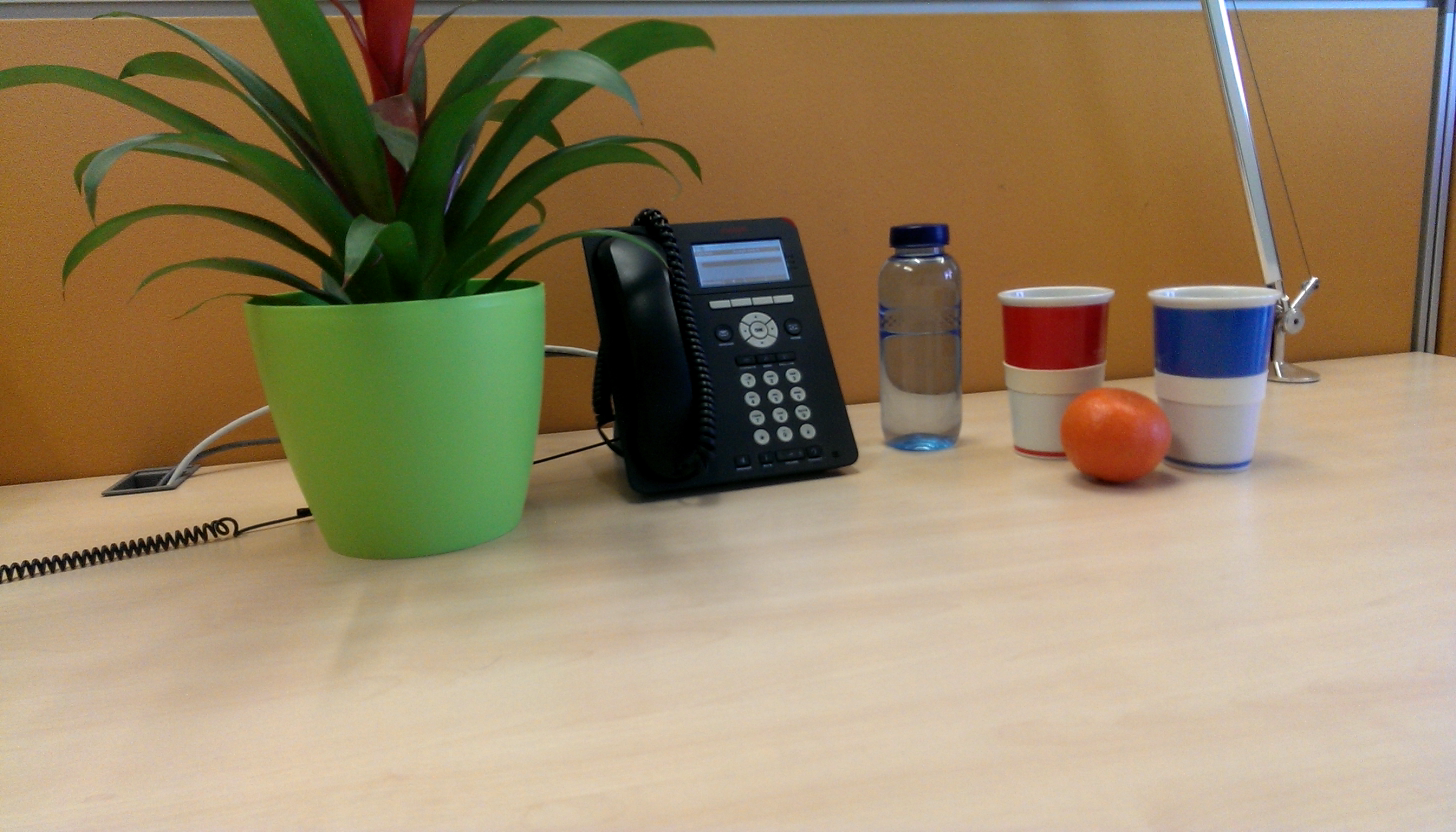
\includegraphics[width=1.4\textwidth]{img/Fotos/QuantiPig_Pixel_1.png}
	\caption[QuantiPig Pixel Modus Intervall 1]{QuantiPig Pixel Modus Intervall 1}
	\label{fig:pig_pix1}
\end{figure}

\begin{figure}[h]
	\centering
		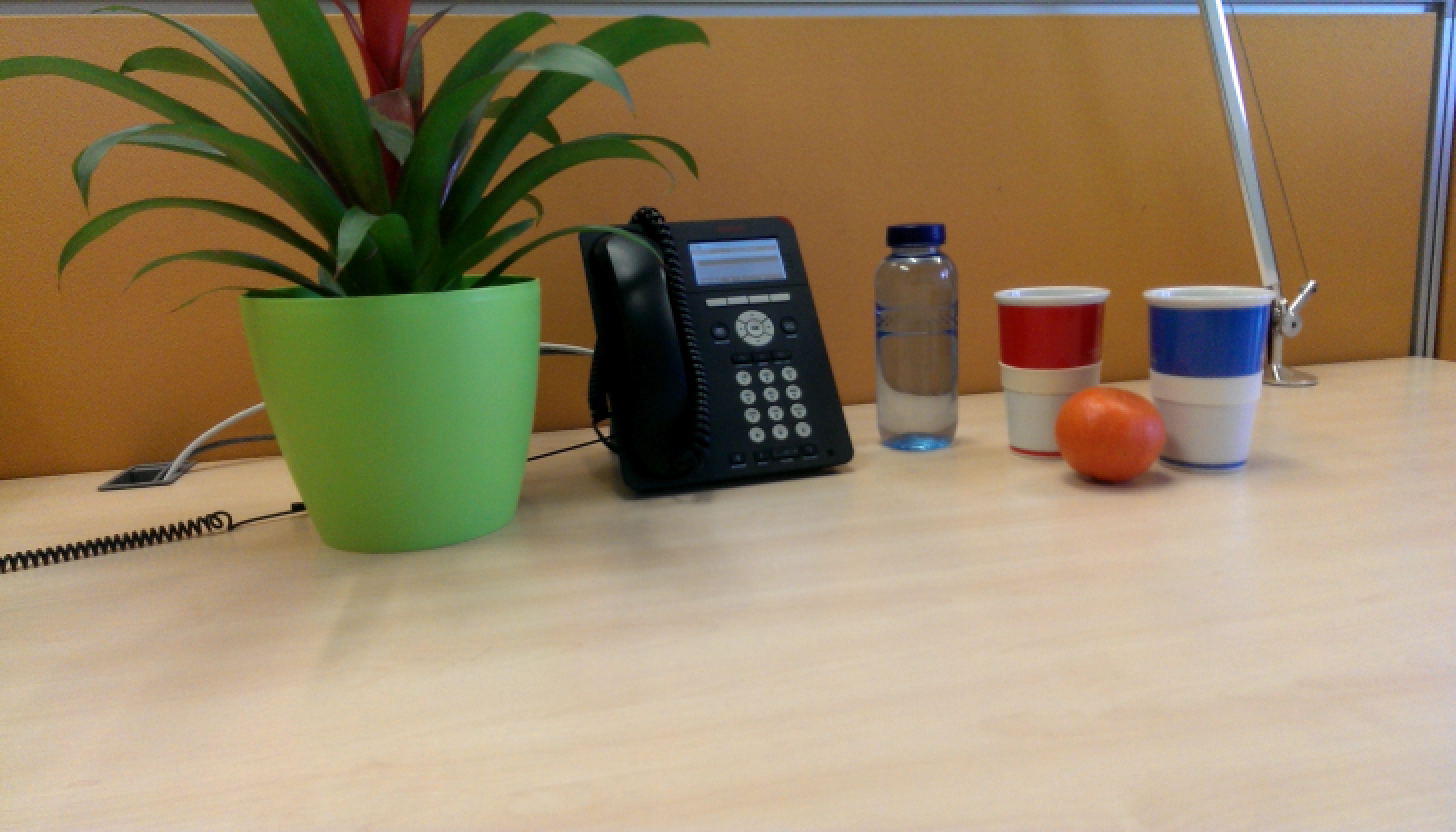
\includegraphics[width=1.4\textwidth]{img/Fotos/QuantiPig_Pixel_2.png}
	\caption[QuantiPig Pixel Modus Intervall 2]{QuantiPig Pixel Modus Intervall 2}
	\label{fig:pig_pix2}
\end{figure}

\begin{figure}[h]
	\centering
		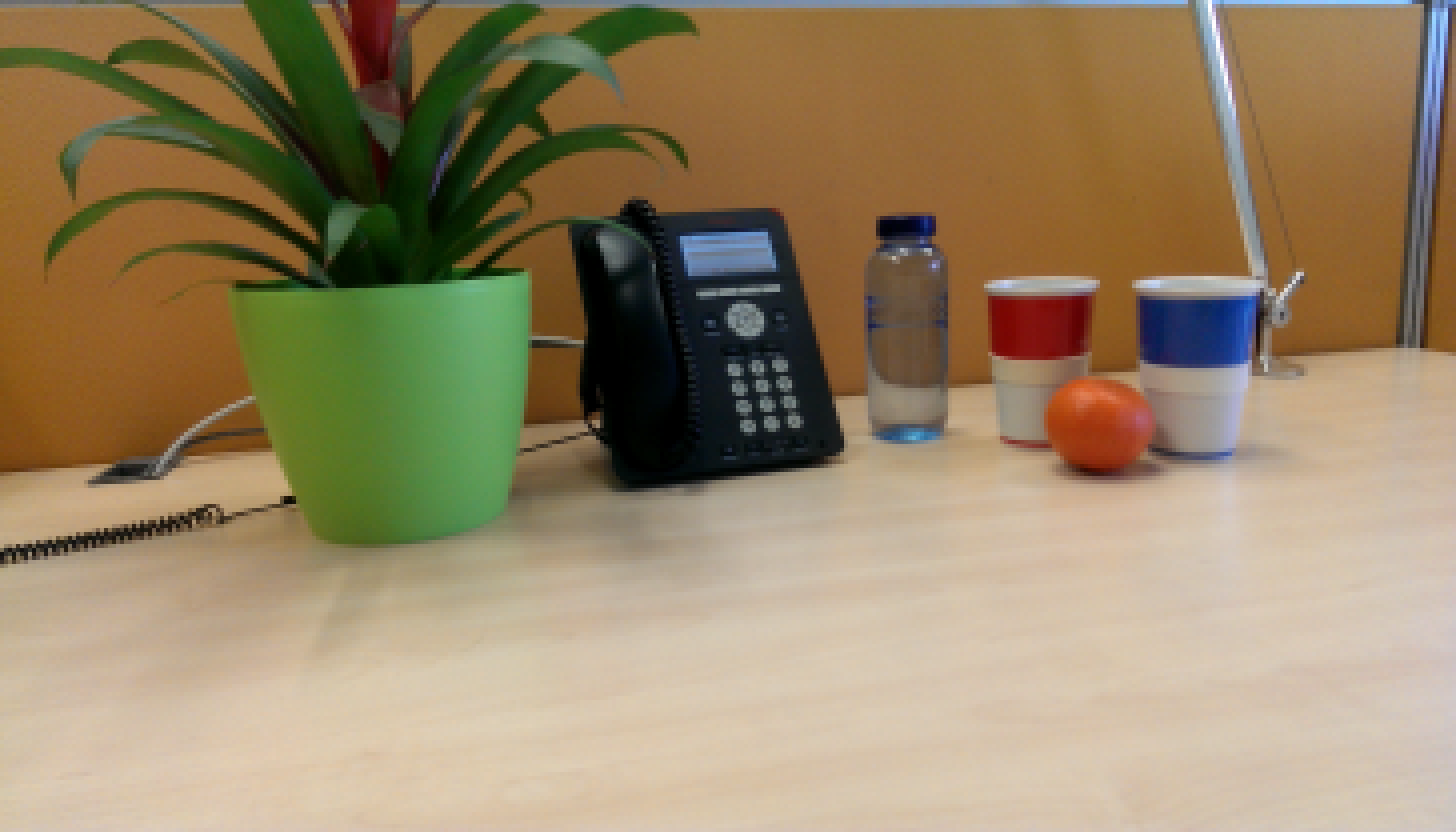
\includegraphics[width=1.4\textwidth]{img/Fotos/QuantiPig_Pixel_4.png}
	\caption[QuantiPig Pixel Modus Intervall 4]{QuantiPig Pixel Modus Intervall 4}
	\label{fig:pig_pix4}
\end{figure}

\begin{figure}[h]
	\centering
		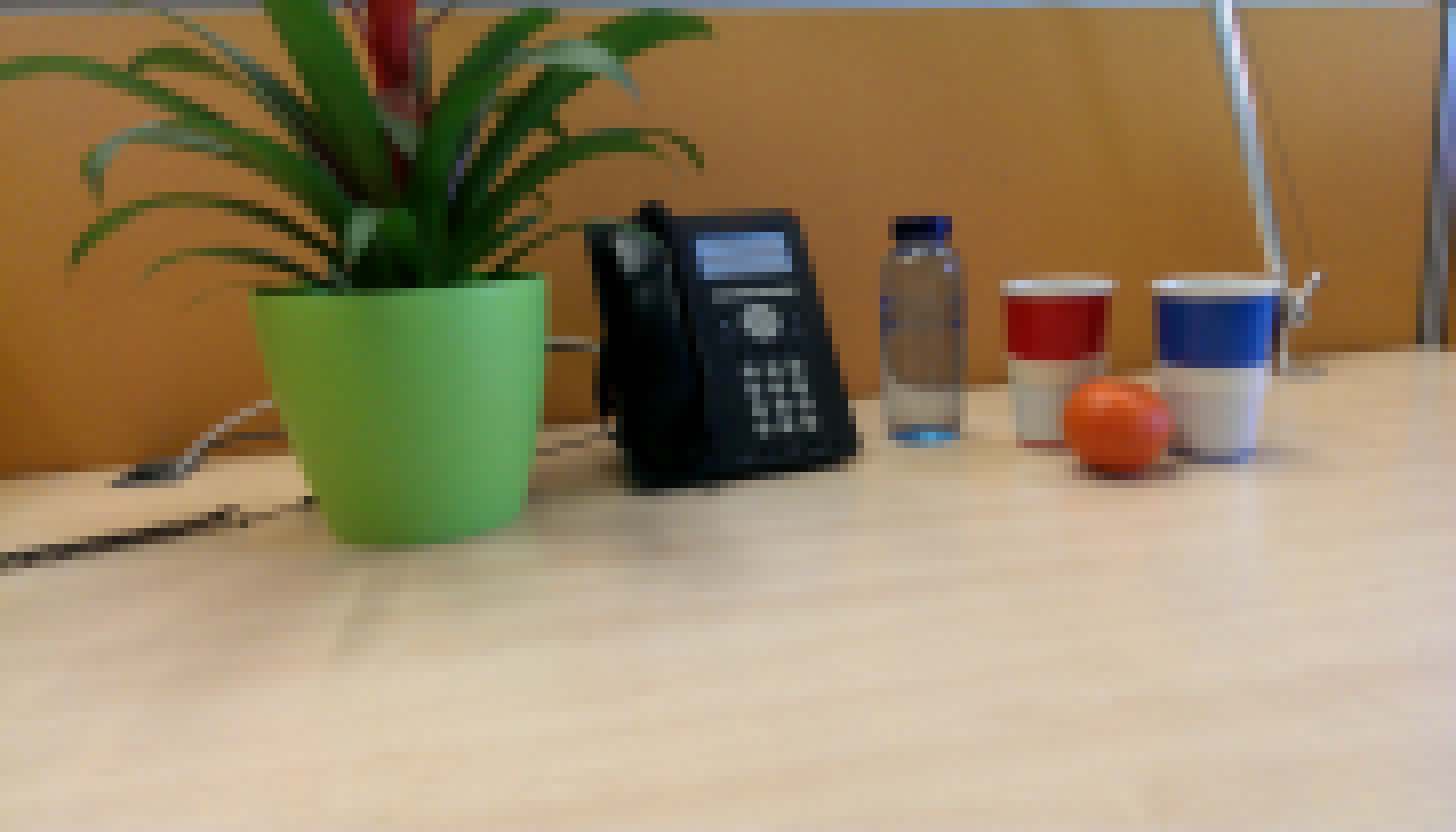
\includegraphics[width=1.4\textwidth]{img/Fotos/QuantiPig_Pixel_8.png}
	\caption[QuantiPig Pixel Modus Intervall 8]{QuantiPig Pixel Modus Intervall 8}
	\label{fig:pig_pix8}
\end{figure}

\begin{figure}[h]
	\centering
		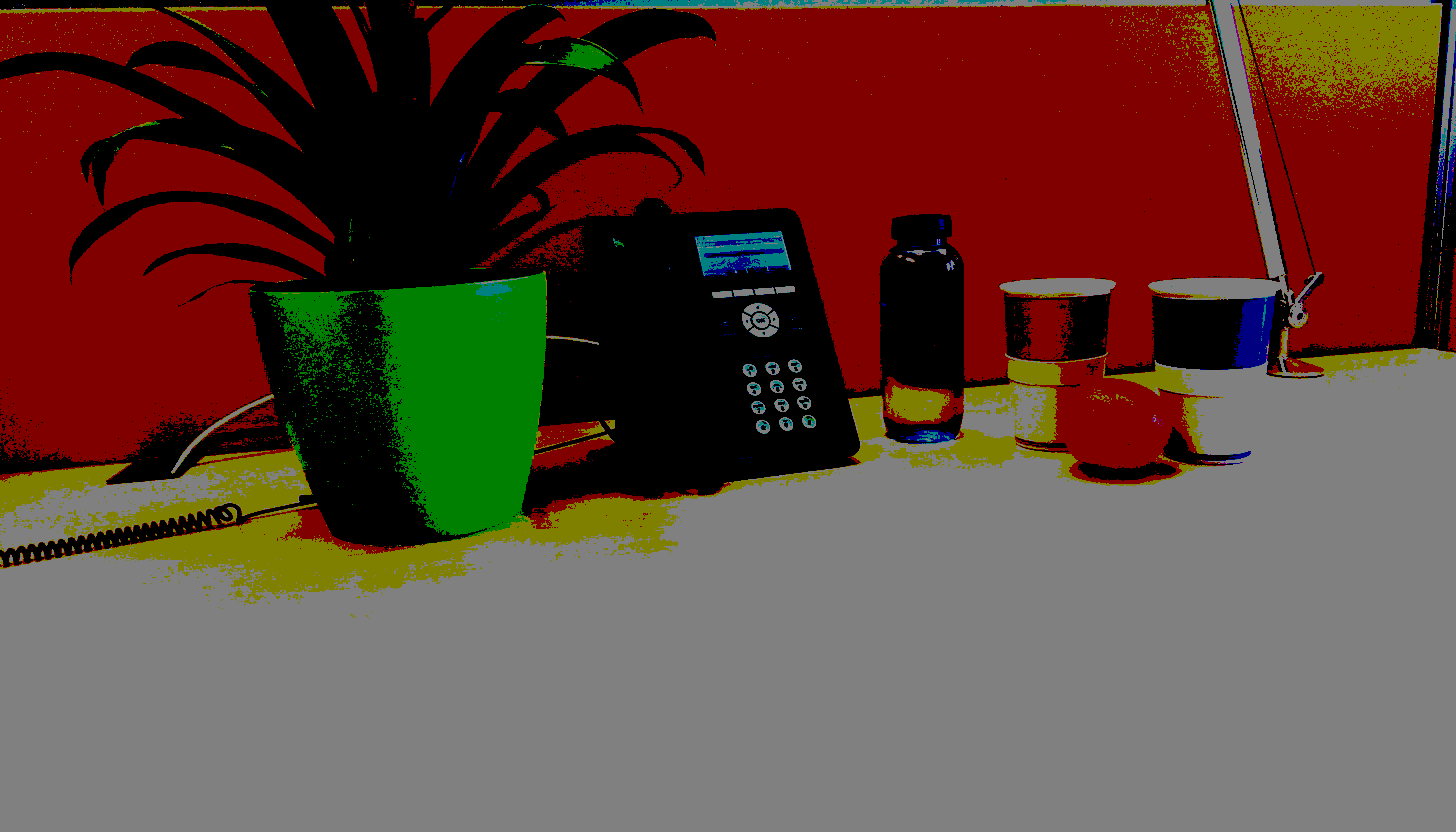
\includegraphics[width=1.4\textwidth]{img/Fotos/QuantiPig_Skalar_1.png}
	\caption[QuantiPig Skalar Modus Intervall 1]{QuantiPig Skalar Modus Intervall 1}
	\label{fig:pig_skal1}
\end{figure}

\begin{figure}[h]
	\centering
		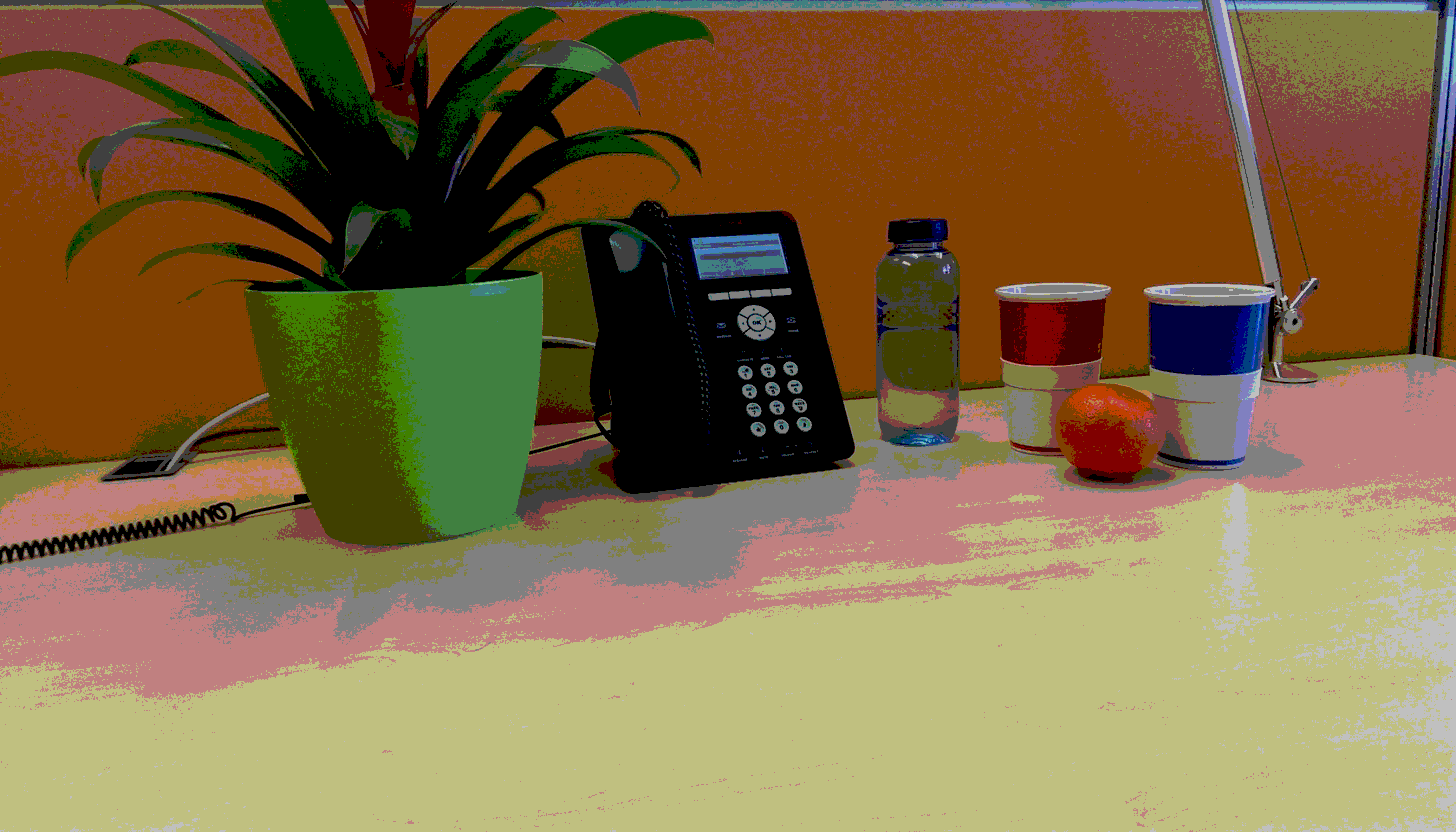
\includegraphics[width=1.4\textwidth]{img/Fotos/QuantiPig_Skalar_2.png}
	\caption[QuantiPig Skalar Modus Intervall 2]{QuantiPig Skalar Modus Intervall 2}
	\label{fig:pig_skal2}
\end{figure}

\begin{figure}[h]
	\centering
		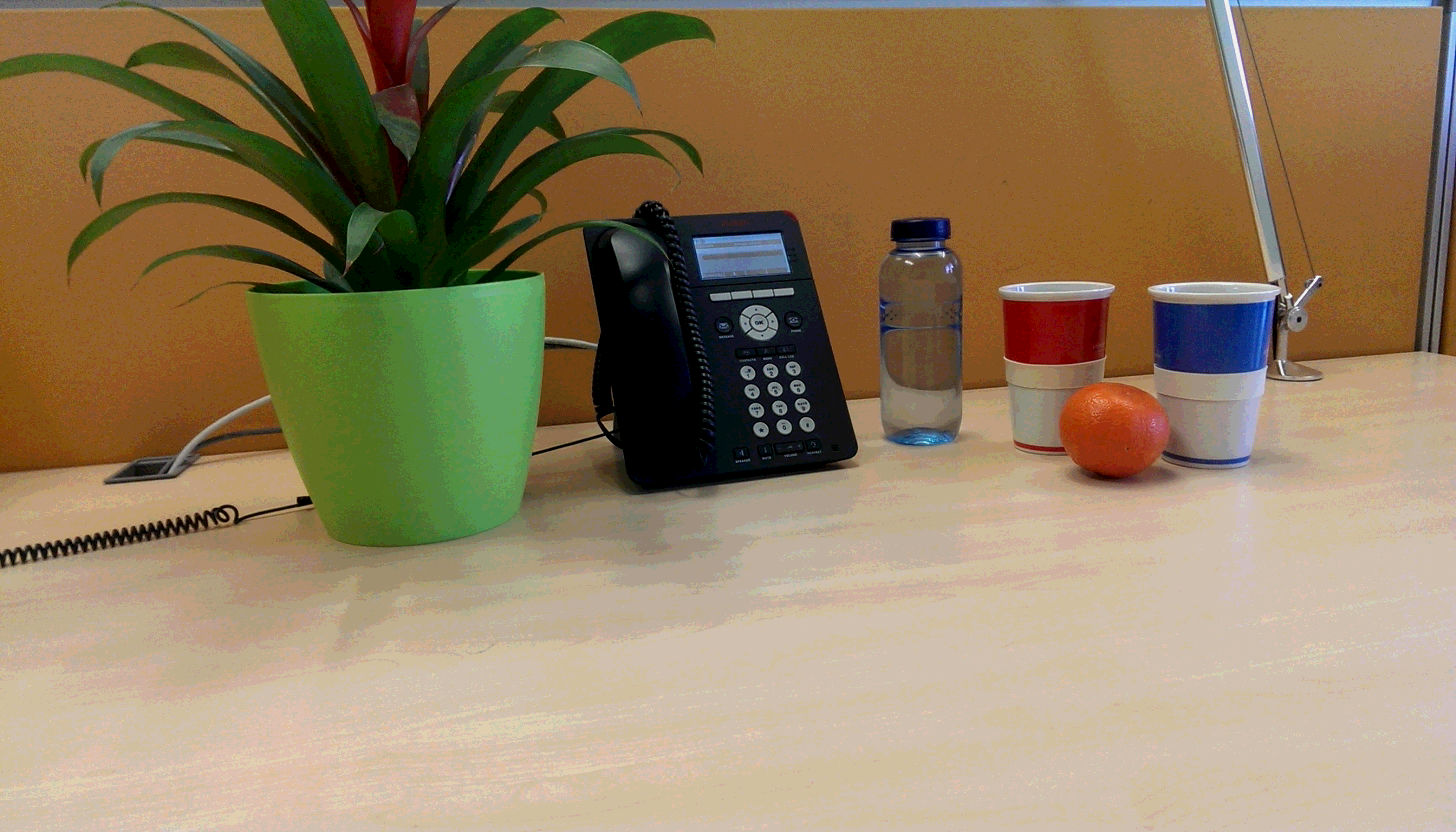
\includegraphics[width=1.4\textwidth]{img/Fotos/QuantiPig_Skalar_4.png}
	\caption[QuantiPig Skalar Modus Intervall 4]{QuantiPig Skalar Modus Intervall 4}
	\label{fig:pig_skal4}
\end{figure}

\begin{figure}[h]
	\centering
		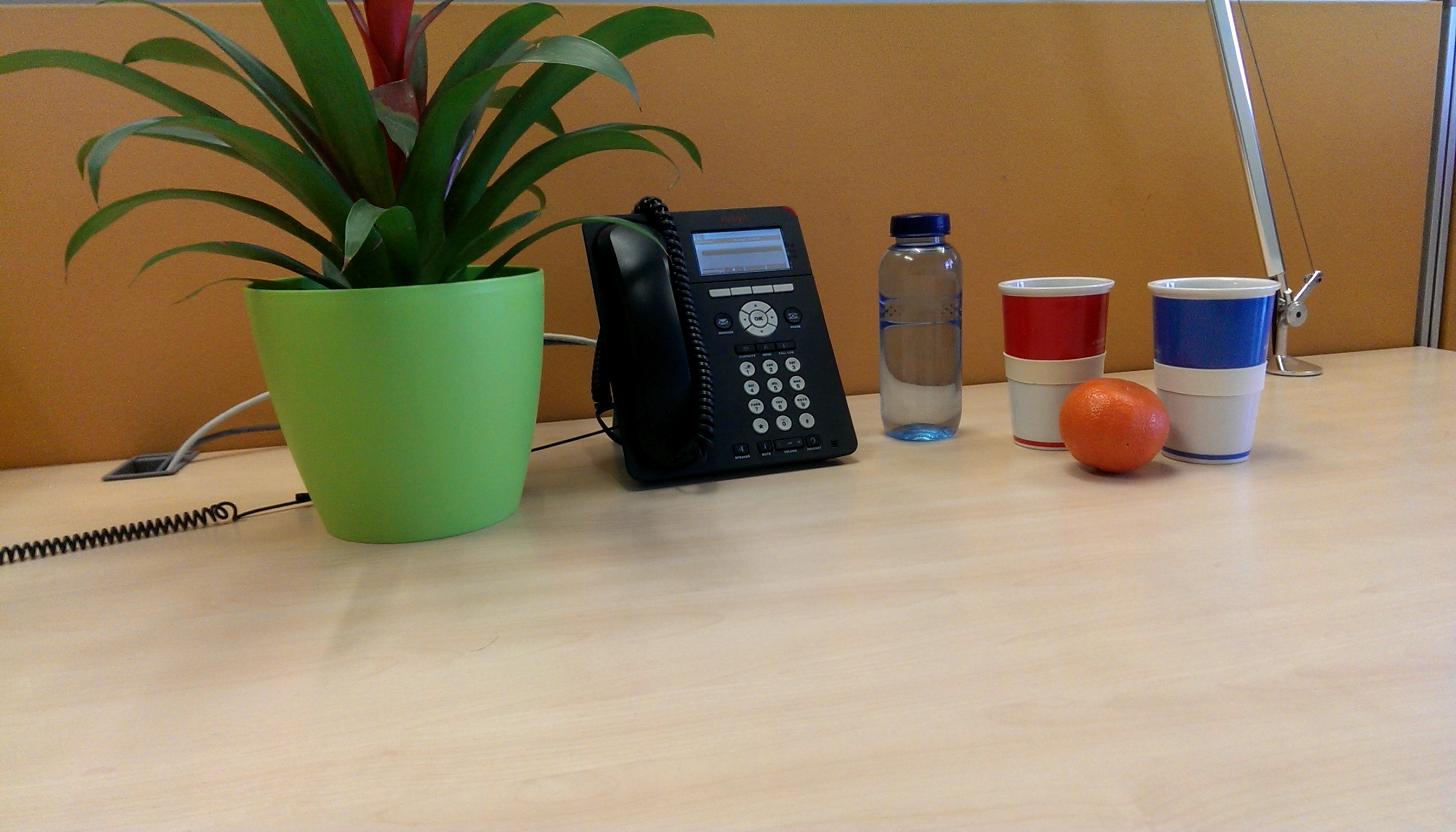
\includegraphics[width=1.4\textwidth]{img/Fotos/QuantiPig_Skalar_8.png}
	\caption[QuantiPig Skalar Modus Intervall 8]{QuantiPig Skalar Modus Intervall 8}
	\label{fig:pig_skal8}
\end{figure}



\end{landscape}


\clearpage


\section{Anhang}

